\documentclass[11pt]{amsart}
\usepackage[a4paper,margin=2.8cm]{geometry}
\usepackage[T1]{fontenc}
\usepackage{newpxtext,newpxmath}
\usepackage{mathtools}
\usepackage{graphicx}
\usepackage{booktabs,array,tabularx}
\usepackage{tikz}
\usetikzlibrary{calc,decorations.markings,arrows.meta}
\usepackage{xcolor}
\usepackage{enumitem}
\usepackage{xurl}
\usepackage[colorlinks=true,linkcolor=blue!50!black,citecolor=green!35!black,urlcolor=blue!50!black,pdftitle={The Spectre Knot: one endless strand on an aperiodic monotile},pdfauthor={Justin Roughley},pdfkeywords={aperiodic monotile, Spectre, substitution tiling, Celtic knot, knot tile, computer-assisted proof, formal verification, Lean}]{hyperref}
\usepackage[capitalise,nameinlink]{cleveref}

\definecolor{oiorange}{HTML}{E69F00}
\definecolor{oisky}{HTML}{56B4E9}
\definecolor{oigreen}{HTML}{009E73}
\definecolor{oiblue}{HTML}{0072B2}
\definecolor{oiverm}{HTML}{D55E00}
\definecolor{oipurple}{HTML}{CC79A7}
\definecolor{ribfill}{HTML}{A6DCC4}
\definecolor{ribedge}{HTML}{0B6B4E}
\definecolor{tilefill}{HTML}{FFF3C4}

\emergencystretch=2em
\newtheorem{theorem}{Theorem}[section]
\newtheorem{lemma}[theorem]{Lemma}
\newtheorem{proposition}[theorem]{Proposition}
\newtheorem{corollary}[theorem]{Corollary}
\newtheorem{computation}[theorem]{Computation}
\newtheorem{mainthm}{Theorem}
\renewcommand{\themainthm}{\Alph{mainthm}}
\newtheorem*{reduction}{Reduction}
\theoremstyle{definition}
\newtheorem{definition}[theorem]{Definition}
\newtheorem{construction}[theorem]{Construction}
\theoremstyle{remark}
\newtheorem{remark}[theorem]{Remark}
\newtheorem{example}[theorem]{Example}
\crefname{mainthm}{Theorem}{Theorems}
\crefname{computation}{Computation}{Computations}
\crefname{construction}{Construction}{Constructions}
\crefname{figure}{Figure}{Figures}

\newcommand{\Tile}{\mathrm{Tile}(1,1)}
\newcommand{\G}{\mathcal G}
\newcommand{\T}{\mathcal T}
\newcommand{\N}{\mathcal N}
\newcommand{\Lp}{\mathrm L}
\newcommand{\Rp}{\mathrm R}
\newcommand{\rim}{\partial}
\newcommand{\ZZ}{\mathbb Z}
\newcommand{\RR}{\mathbb R}
\newcommand{\code}[1]{\texttt{#1}}
\newcommand{\Fib}{F}

\title[The Spectre Knot]{The Spectre Knot:\\ one endless strand on an aperiodic monotile}
\author{Justin Roughley}
\address{Independent researcher}
\email{cortado.just@gmail.com}
\date{22 October 2026}
\subjclass[2020]{Primary 52C20; Secondary 05B45, 52C23, 57K10, 68V05, 68V20}
\keywords{aperiodic monotile, Spectre, substitution tiling, Celtic knot, knot tile, computer-assisted proof, formal
verification, Lean}

\begin{document}

\begin{abstract}
The Spectre of Smith, Myers, Kaplan and Goodman-Strauss tiles the plane, but only non-periodically. We decorate its
straight-edged form $\Tile$ with fourteen ribbon pieces, the same on every tile, so that the ribbons continue straight
across every tile edge. We prove two theorems. In every tiling by copies of $\Tile$ of one handedness whose supertile
hierarchy covers the plane, no strand of ribbon is closed. In the \emph{nest tiling}, grown outwards from a single tile
through $\Delta$-supertiles, each block sitting in the same place (child number~$1$) inside the next, all the pieces
join into a single strand, a two-way infinite path through every tile; we do not claim this for other tilings. Every
supertile connects the ribbon ends on its boundary in one and the same pattern, with no closed strand inside; ribbons
zigzag along a boundary shared by two supertiles, so lengthening it by two edges changes nothing; and the side lengths
at every level are reached from those at level~$1$ by such two-edge steps. So finitely many computations at level~$1$
settle every level. The combinatorial core is formalised in the Lean proof assistant. At the author's instruction, an
AI system generated the proof, the programs, the formalisation, the figures and this text. This paper has not been peer
reviewed.
\end{abstract}

\maketitle

% ---------------------------------------------------------------------------------------------------------
\section{Introduction}\label{sec:intro}

A \emph{Celtic knot} is a pattern of interlaced ribbons~\cite{Bain,Cromwell1993}; the number of strands in finite
designs of this kind has been studied, for instance, by Fisher and Mellor~\cite{FisherMellor}. A \emph{knot tile} is a
polygon carrying ribbon pieces that end on its edges, so that when copies of the tile are placed edge to edge, the
pieces join up into longer ribbons; knot mosaics~\cite{LomonacoKauffman} assemble knot diagrams in this way from a set
of square tiles. We ask for a knot tile whose ribbons, in a tiling of the whole plane, form one endless strand. In a
periodic tiling this cannot happen. Suppose that the pieces formed one strand. Each piece has two ends, each joined to
exactly one other piece, so the strand is a two-way infinite path $\dots,p_{-1},p_0,p_1,\dots$, and a period $\tau$ of
the decorated tiling (for a tile with no symmetry, such as $\Tile$, every period of the tiling is one) maps it onto
itself, keeping joins: it shifts it, $p_i\mapsto p_{i+k}$, or reverses it, $p_i\mapsto p_{c-i}$. A reversal is
impossible, since $\tau^2$ would then fix every piece, but $\tau^2$ moves every tile; for the same reason $k\neq0$. The
pieces would then form $|k|$ orbits under $\langle\tau\rangle$, whereas the tiles form infinitely many, as
$\RR^2/\langle\tau\rangle$ has infinite area and the tiles of one orbit cover at most the area of one tile there; and
tiles in different orbits carry pieces in different orbits.
So we look at a tile that tiles only non-periodically.

Socolar and Taylor~\cite{SocolarTaylor} found a hexagonal tile that, with its mirror image, tiles only
non-periodically when its markings are matched. In 2023 Smith, Myers, Kaplan and Goodman-Strauss described the
\emph{hat}, an aperiodic monotile~\cite{SMKGS-hat}, and then the \emph{Spectre}~\cite{SMKGS-spectre}: a shape that
tiles the plane, but only non-periodically and, even when reflections are allowed, only with all tiles of the same
handedness~\cite[Thm.~2.2]{SMKGS-spectre}. The Spectre is a curved-edge form of the polygon $\Tile$, and tilings by
Spectres correspond exactly to the tilings by $\Tile$ with all tiles of one handedness (\cref{fig:tile},
\cref{sec:spectre}). For background on tilings and substitution see~\cite{GrunbaumShephard,BaakeGrimm}.

We give a knot tile on the Spectre that is \emph{mono-stranded}: in one explicit tiling the pieces of all the tiles
form a single strand (\cref{thm:B}). Moreover, no tiling whose supertile hierarchy covers the plane (defined below)
contains a closed strand (\cref{thm:A}). The decoration (\cref{fig:tile}) puts one crossing point on each of the
fourteen edges, with two ribbon ends at each, and joins these $28$ ends in pairs inside the tile by fourteen pieces:
twelve \emph{hooks}, each turning back round one vertex, and two pieces that cross each other once. Across an edge,
the ribbons continue straight through the crossing point.

\begin{figure}[t]
\centering
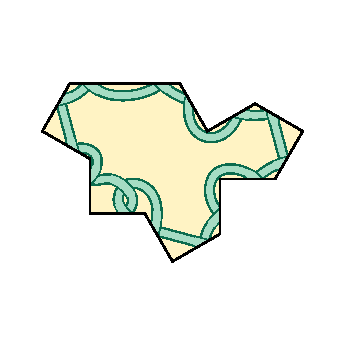
\includegraphics[width=0.19\textwidth]{figs/tile_ribbons.pdf}\hfill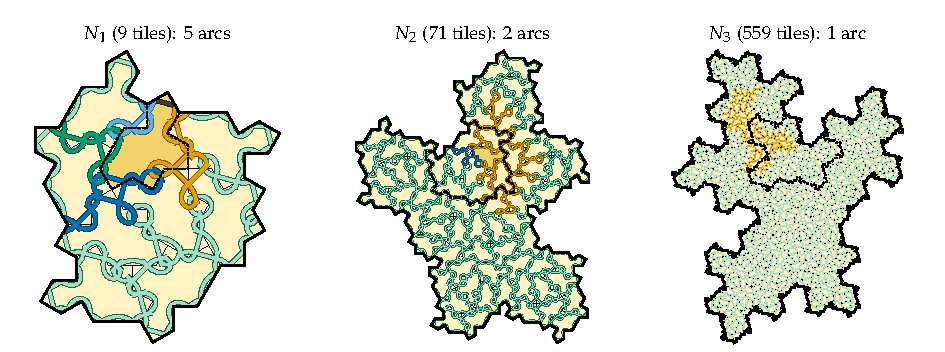
\includegraphics[width=0.79\textwidth]{figs/merge.pdf}
\caption{Left: the tile $\Tile$ with its fourteen ribbon pieces. Right: the blocks $N_1$, $N_2$, $N_3$ of the nest
tiling (\cref{sec:nest}), each drawn with the previous block, its child number~$1$, dashed. The pieces of the original
tile $N_0$ (shaded) lie on $5$ arcs of $N_1$, $2$ of $N_2$ and $1$ of $N_3$ (\cref{tab:merge}, row $b=0$), one colour
per arc; an arc is a ribbon path through the block from boundary to boundary (\cref{sec:boxes}).}
\label{fig:tile}
\end{figure}

Every tiling by $\Tile$ with tiles of one handedness (a \emph{homochiral} tiling) groups uniquely into a hierarchy of
larger and larger \emph{supertiles}~\cite[Thm.~2.2]{SMKGS-spectre}. We say that the hierarchy \emph{covers the plane}
if the supertiles containing some tile exhaust the plane. This does not depend on the tile: if the supertiles containing a
tile $t$ exhaust the plane, one of them contains an interior point of any other tile $t'$, and so contains $t'$
(supertiles are unions of tiles, and distinct tiles have disjoint interiors); from that level on, $t$ and $t'$ have
the same supertiles. If the hierarchy does not cover
the plane, the tiling splits into two or more \emph{infinite supertiles}, unions of nested chains of supertiles,
separated by a \emph{fault} (\cref{sec:scope}).

\begin{mainthm}[The Daedalus Theorem]\label{thm:A}
In every homochiral tiling of the plane by $\Tile$ whose supertile hierarchy covers the plane, with every tile carrying
the decoration of \cref{fig:tile} (\cref{def:decoration}), there is no closed strand: every strand is a two-way
infinite path of ribbon pieces.
\end{mainthm}

Our second result is proved for one tiling, the \emph{nest tiling} $\N$, grown from a single tile $N_0$ by repeatedly
taking the $\Delta$-supertile $N_{b+1}$ that has $N_b$ as its child number~$1$ (\cref{sec:nest}); the $N_b$ are its
\emph{blocks}, and an \emph{arc} of a block is a path of its ribbon pieces with both ends on its boundary
(\cref{lem:box}). In the language of substitution tilings, $\N$ is generated from one tile by iterating the
substitution about it, and is a fixed point of the substitution in the combinatorial sense (compare~\cite{BaakeGrimm}).
In the tile addresses of~\cite[\S2.8]{TathamTransducers} (after~\cite{GoodmanStrauss1999}), $N_0$ has the address
\[
\Delta\xleftarrow{1}\Delta\xleftarrow{1}\Delta\xleftarrow{1}\cdots.
\]

\begin{mainthm}[The Ariadne Theorem]\label{thm:B}
In the nest tiling $\N$, with every tile carrying the decoration of \cref{fig:tile} (\cref{def:decoration}), all the
ribbon pieces of all the tiles form a single strand. It is a two-way infinite path that passes through every tile. More
precisely, for every $b\ge 1$, all the pieces of the block $N_b$ lie on a single arc of $N_{b+3}$ if $b$ is even, and
of $N_{b+4}$ if $b$ is odd.
\end{mainthm}

We make no claim about the number of strands in any other tiling: computations indicate that in at least one other
tiling whose hierarchy covers the plane, the pieces of a level-$1$ supertile lie on three strands. Tilings with faults
are covered by neither theorem (\cref{sec:scope}).

The names recall the myth: Daedalus built the labyrinth, in which no strand closes (\cref{thm:A}); Ariadne gave the
thread, which runs through every tile of $\N$ (\cref{thm:B}).

\subsection*{The method}
The proof has three ideas.
\begin{enumerate}[leftmargin=*]
\item \emph{Black boxes.} Seen from outside, a supertile is just a list of which ribbon end on its boundary is
joined to which. Every supertile of every kind and level $m\ge1$ has the same \emph{signature} as a single tile: a hook
at every tile vertex on its boundary but two adjacent ones, the crossover corners $A$ and $B$, where two ribbons cross
over; and no closed strand inside (\cref{def:signature}, \cref{thm:signature}, \cref{fig:signature}).
\item \emph{Zigzags.} When two such boxes are glued along a common boundary path with no crossover corner inside it,
the ribbons zigzag along it, and how they join the two ends of the path depends only on the parity of its length
(\cref{lem:zigzag}). So lengthening a shared path by two edges changes nothing (\cref{lem:lengthen}).
\item \emph{Fixed parities.} The supertiles are combinatorially hexagons and compose by the substitution
of~\cite[Fig.~5.1]{SMKGS-spectre}. Their side lengths are given by Fibonacci numbers (\cref{prop:fib}), grow with the
level and never change parity. So the side lengths at any level are reached from those at level~$1$ by lengthening,
two edges at a time (\cref{lem:reach}). By induction on the level, a supertile is glued from children that already
have the signature, so its box is that of a composition of boxes, fixed by its kind, the side lengths and where the
children's corners $A$ and $B$ lie (\cref{sec:comp}); the $18$ compositions at the level-$1$ lengths (nine kinds, $B$
on either side of $A$), computed once, give the signature at every level.
\end{enumerate}
A closed strand is finite, so when the hierarchy covers the plane it lies in one supertile, where the signature forbids
it; this gives \cref{thm:A}. The single strand (\cref{thm:B}) follows the same pattern. Unlike the signature, this
uses how each block sits in the next (as child~$1$). In the next block up, every arc of a block lies on a hook (an arc
with both ends at one boundary vertex), and which hook depends only on where the arc meets the boundary; for vertices
well inside five of the six sides, only on the side (\cref{lem:junctionmap}, \cref{tab:junction}). This \emph{junction
map} is computed at level~$1$ and carried to every level by the same lengthening. Followed three or four levels up, it
puts all the arcs of a block on one arc (\cref{thm:merge}).
The finite computations (the level-$1$ data and \cref{comp:base}; \cref{comp:compose} on the $18$ compositions at the
level-$1$ lengths, and \cref{comp:junction} on two of them) are exact; \cref{comp:compose,comp:junction} are repeated in the
kernel of the Lean proof assistant, and so is \cref{comp:base}, on the level-$1$ supertiles of \code{exact.py}, with their corner
$A$, taken as input. The agreement with~\cite[Figs.~4.1, 5.1]{SMKGS-spectre} is
checked by scripts, against a render of Fig.~4.1, whose labels were transcribed from the figure, and against an
encoding of Fig.~5.1 (\cref{app:computations}). \Cref{fig:roadmap} shows how the steps fit together, and which of them Lean checks.

\begin{figure}[t]
\centering
\definecolor{oiyellow}{HTML}{F0E442}
\begin{tikzpicture}[x=1cm,y=1cm,font=\scriptsize,
  box/.style={draw=black!70,rounded corners=2pt,align=center,inner sep=2pt,minimum height=0.9cm,text width=3.4cm,
    execute at begin node={\hyphenpenalty=10000\exhyphenpenalty=10000}},
  lean/.style={box,fill=oiyellow!40},
  word/.style={box,fill=white,densely dashed},
  part/.style={box,fill=oiyellow!40,densely dashed},
  arr/.style={-{Stealth[length=4pt]},black!65,line width=0.5pt}]
\node[word] (smkgs) at (0,3.6)     {Spectre hierarchy, cited (Thm.~\ref{thm:smkgs}); the pattern at every level (Prop.~\ref{prop:pattern}); rigidity (Lemma~\ref{lem:rigid})};
\node[lean] (box)   at (0,1.7)    {Boxes and the signature (\S\ref{sec:boxes})};
\node[lean] (fib)   at (0,0)       {Side lengths are given by Fibonacci numbers and never change parity (\S\ref{sec:lengths})};
\node[lean] (comp)  at (3.95,3.6)  {Level $1$: the $18$ compositions and the base, computed (Comps.~\ref{comp:compose}, \ref{comp:base})};
\node[lean] (zig)   at (3.95,1.7) {Zigzag Lemma~\ref{lem:zigzag}: only parity matters; two-edge moves keep the signature (Lemma~\ref{lem:lengthen}) and reach every level (Lemma~\ref{lem:reach})};
\node[part] (A)     at (7.9,3.6)   {\textbf{Theorem A}: no closed strand if the hierarchy covers the plane};
\node[lean] (sig)   at (7.9,1.7)  {\textbf{Signature Theorem~\ref{thm:signature}}: every supertile has the signature};
\node[lean] (junc)  at (7.9,0)     {Junction map, at level $1$ and every level (Comp.~\ref{comp:junction}; Lemmas~\ref{lem:junctionmap}, \ref{lem:junctions})};
\node[part] (nest)  at (11.85,3.6) {The nest tiling covers the plane (\S\ref{sec:nest}; Grandparent Lemma~\ref{lem:gap})};
\node[part] (B)     at (11.85,1.7) {\textbf{Theorem B}: one strand in the nest tiling};
\node[lean] (merge) at (11.85,0)   {Merging: the arcs of $N_b$ lie on one arc of $N_{b+4}$, of $N_{b+3}$ if $b$ is even (Thm.~\ref{thm:merge})};
\draw[arr] (smkgs) -- (comp);
\draw[arr] (box) -- (zig);
\draw[arr] (fib.east) -- (zig.south west);
\draw[arr] (comp) -- (sig);
\draw[arr] (zig) -- (sig);
\draw[arr] (sig) -- (A);
\draw[arr] (sig) -- (junc);
\draw[arr] (zig.south east) -- (junc.north west);
\draw[arr] (junc) -- (merge);
\draw[arr] (merge) -- (B);
\draw[arr] (nest) -- (B);
\draw[arr] (smkgs.north) -- ++(0,0.32) -| (nest.north);
\coordinate (top) at ($(smkgs.north)+(0,0.32)$); \draw[arr] (A.north |- top) -- (A.north);
\end{tikzpicture}
\caption{The route of the proof. Shaded: checked by the Lean formalisation in a combinatorial form, including the
computations at level~$1$ (\cref{comp:base} on the level-$1$ supertiles of \code{exact.py}, with their corner $A$, taken as input). Dashed: the
link with actual tilings, cited from~\cite{SMKGS-spectre} or argued in words. Shaded and dashed: Lean checks the
combinatorial part, and the link with actual tilings is argued in words (\cref{app:ai}).}
\label{fig:roadmap}
\end{figure}

\subsection*{Organisation}
\Cref{sec:spectre} recalls the hierarchy of~\cite{SMKGS-spectre}, in our numbering. \Cref{sec:decoration} defines the
decoration and its strands, and \cref{sec:boxes} introduces boxes and the signature. \Cref{sec:reduce} proves the
Zigzag Lemma, \cref{sec:lengths} finds the side lengths, and \cref{sec:induction} proves the Signature Theorem and
\cref{thm:A}. \Cref{sec:nest} constructs the nest tiling and shows that it covers the plane, and \cref{sec:strand}
proves \cref{thm:B}. \Cref{sec:scope} discusses scope and open questions; \cref{app:computations} describes the
computations, and \cref{app:ai} the use of AI, the formal verification and the tools.

\subsection*{Related work}
Curves drawn on tiles and joined across edges, each closed or two-way infinite as in \cref{lem:degree2}, have been
studied for random Truchet tilings~\cite{Pete2008,Hooper2011} and for a deterministic family of them, in which a
renormalisation, akin to our induction on supertiles, shows that for almost every parameter almost every curve is
closed~\cite{Hooper2013}. Mirror curves of Celtic, Tchokwe and Tamil designs are another
case~\cite{Gerdes2007,JablanKnotsArt}: a design drawn as a single line is called \emph{monolinear}, and a rectangular
grid of $m\times n$ cells with no inner mirrors carries $\gcd(m,n)$ curves~\cite{Gerdes2007}. So are the
Conway--Penrose arcs on Penrose tiles, where at most two curves of each colour fail to close~\cite[Ch.~1]{Gardner1989}
(see also~\cite{FlickerSimonParameswaran}), and girih interlace on Penrose tilings, whose strands close into loops and
knots~\cite{Cline2024,Cline2025,Gaenshirt2024}. Single curves through finite patches have been built as Hamiltonian
cycles, through every vertex of arbitrarily large regions of Ammann--Beenker tilings~\cite{SinghLloydFlicker} and through every
tile of finite Penrose and Ammann--Beenker patches~\cite{LiuChoiMahadevan}, and as space-filling curves from aperiodic
substitution tilings~\cite{Pautze2021}. Closest to this paper, an online project~\cite{BohemianMiserSpectre} decorates
selected edges of $\Tile$ and describes a single non-crossing curve through every tile of one nested tiling, with a
machine check of the combinatorial core of its argument. Here every edge carries a crossing point, and two pieces
cross inside each tile. In our drawing every crossing is a transversal double point (\cref{app:computations}), so over
and under can alternate by the checkerboard rule~\cite{CromwellKnots}, and the single strand becomes an alternating
diagram of a line. Celtic knotwork is alternating in the same way, and up to topological equivalence its designs
realise every alternating link projection~\cite{GrossTucker}.
We are not aware of earlier full knotwork decorations that form a single strand.

\subsection*{Use of AI and verification status}
This work is an experiment in using AI for mathematical exploration. At the author's instruction, an AI system
(Claude, by Anthropic) generated the programs, the proofs, the Lean formalisation, the figures and this text; the
author asked the question, steered the work, made the choices and decisions, corrected what was generated, and answers
for the work.
The author is responsible for the paper: for the correctness of its arguments and results, and for the completeness and
accuracy of its citations of prior work. The AI system is not an author. Lean checks the combinatorial core of the
proof; the link with actual tilings is argued in words. Most of the proof has not been reviewed by a human, and the
paper has not been peer reviewed. \Cref{app:ai} gives the full account: how the work was done, what the formalisation
checks, and the tools used.

% ---------------------------------------------------------------------------------------------------------
\section{Spectre tilings}\label{sec:spectre}
\suppressfloats[t]

The proof climbs the supertile hierarchy of~\cite{SMKGS-spectre} one level at a time. This section fixes what it uses:
the tile, its supertiles (\cref{thm:smkgs}), an orientation, a side numbering and a crossover corner for each supertile
(\cref{sec:own}), and the tables by which each level from level~$2$ up is assembled from the one below
(\cref{sec:pattern}). The decoration enters in \cref{sec:decoration}; the tables are first used in \cref{sec:lengths},
and a first reading may postpone their details until then.

\begin{center}\footnotesize
\begin{tabular}{@{}l@{\enspace}l@{\hspace{2em}}l@{\enspace}l@{}}
\toprule
\multicolumn{4}{@{}l}{\emph{Notation}}\\
\midrule
$\Tile$, $v_i$, $e_i$; homochiral tiling $\T$ & \cref{sec:tile} &
rim ports $\Rp(u_k)$, $\Lp(u_k)$ & \cref{sec:boxes}\\
kinds $K$, levels $m$, children, $n_T$ & \cref{sec:supertiles} &
$\pi_P$, arcs, boxes, closed strands of $P$ & \cref{lem:box}\\
rim, vertices, sides, rim vertices & \cref{sec:supertiles} &
signature at $(A,B)$ & \cref{def:signature}\\
own orientation, own order, $\omega_m$ & \cref{def:own} &
$\ell_m(K,j)$ & \cref{sec:lengths}\\
crossover corners $A$, $B=A+\omega_m$ & \cref{sec:own} &
letters $\alpha,\dots,\theta$ & \cref{sec:lengths}\\
parent kind $T$, child kinds $K_c$ & \cref{def:pattern} &
lengths $\alpha_m,\dots,\theta_m$ & \cref{prop:letters}\\
child $c$, child side $c.j$, parent side $J$ & \cref{tab:sides,tab:psides} &
$d_m$ & \cref{lem:Apos}\\
ports $\Rp(v_i)$, $\Lp(v_i)$ & \cref{sec:decoration} &
$C_T(L,d,\omega)$, $A_c$, $B_c$, $c_\Sigma$, $A_\Sigma$, $A_\Gamma$ & \cref{sec:comp}\\
pieces, hooks, crossover & \cref{def:decoration} &
moves, admissible pairs & \cref{sec:lengthen}\\
strands, closed strands, $\G(\T)$ & \cref{def:strandgraph} &
nest tiling $\N$, blocks $N_b$ & \cref{sec:nest}\\
patch $P$, its rim $\rim P$, $E=E(P)$ & \cref{sec:boxes} &
junctions $q$, hooks $H_q$ & \cref{sec:junctions}\\
\bottomrule
\end{tabular}
\end{center}

\subsection{The tile}\label{sec:tile}
Let $\rho=e^{i\pi/6}$. The polygon $\Tile$ has fourteen unit edges; we label its vertices $v_0,\dots,v_{13}$
anticlockwise (\cref{fig:tileports}, left) and its edges $e_i=v_iv_{i+1}$ (indices mod $14$), with $v_0=0$ and
\[
v_{i+1}-v_i=\rho^{k_i},\qquad (k_0,\dots,k_{13})=(0,10,1,3,0,2,5,7,4,6,6,8,11,9).
\]
All vertices lie in $\ZZ[\rho]$. $\Tile$ is the equilateral member of the family $\mathrm{Tile}(a,b)$~\cite[\S\S1--2]{SMKGS-spectre},
with its long side split into the collinear edges $e_9,e_{10}$. It is the mirror image of the polygon drawn
in~\cite[Fig.~1.1]{SMKGS-spectre} and has the handedness of the single Spectre and of the Mystic
in~\cite[Fig.~2.1]{SMKGS-spectre}. A tiling by $\Tile$ is \emph{homochiral} if any two of its tiles are related by a
\emph{proper motion} (a rotation followed by a translation). \emph{Spectres} are tiles whose tilings correspond exactly
to the homochiral tilings by $\Tile$, each Spectre placed by the same isometry as the corresponding copy of
$\Tile$~\cite[\S2, Lemma~2.1]{SMKGS-spectre}; one is obtained by replacing every edge of $\Tile$ by a suitable curve. So
what~\cite{SMKGS-spectre} proves for tilings by Spectres holds for homochiral tilings by $\Tile$~\cite[p.~5]{SMKGS-spectre}.
Such tilings exist~\cite[Thm.~2.2]{SMKGS-spectre}, and in each, tiles meet full edge to full edge~\cite[proof of
Lemma~2.1]{SMKGS-spectre}. Reflecting the plane if necessary, we assume that every tile is the image of $\Tile$ under a
rotation and a translation; a reflection carries the decoration of each tile (\cref{def:decoration}) to that of its
image, and so strands to strands. The tile has no non-trivial symmetry, proper or improper (its turning angles at
$v_1,\dots,v_{13},v_0$, in units of $30^\circ$, are $-2,3,2,-3,2,3,2,-3,2,0,2,3,-2,3$; the only $0$ is at $v_{10}$, and
the sequence is not symmetric about it), so an isometry between two tiles is unique.

\subsection{Supertiles}\label{sec:supertiles}
We use the hierarchy of~\cite{SMKGS-spectre}, with nine \emph{kinds} $\Gamma,\Delta,\Theta,\Lambda,\Xi,\Pi,\Sigma,\Phi,\Psi$.
A \emph{level-$0$ supertile} of kind $K\neq\Gamma$ is a single tile; one of kind $\Gamma$ is a
\emph{Mystic}~\cite[Fig.~2.1]{SMKGS-spectre} (the darker pair of tiles in \cref{fig:level1}): a pair of tiles
$\{h(\Tile),\ h(g(\Tile))\}$, where $g(z)=\rho z+v_8$ and $h$ is a proper motion, with \emph{first} tile $h(\Tile)$. The
first tile is determined by the pair, since the Mystic has no non-trivial proper symmetry: a symmetry exchanging its
tiles would be an involution taking $\Tile$ to $g(\Tile)$, but the only proper motion doing so is $g$, a rotation by
$30^\circ$. A level-$(m+1)$ supertile of kind $T$ is the union of level-$m$ supertiles, its $n_T$ \emph{children}, of
the kinds listed in \cref{tab:children}, where $n_\Gamma=7$ and $n_T=8$ for $T\neq\Gamma$. A level-$1$ supertile has the
kind of its cluster in~\cite[Fig.~4.1]{SMKGS-spectre}; the positions of its six vertices (\cref{fig:level1}) determine
that kind~\cite[proof of Thm.~4.1]{SMKGS-spectre}; a level-$(m+1)$ supertile, $m\ge1$, has kind $T$ if its children form
the panel $T$ of~\cite[Fig.~5.1]{SMKGS-spectre} (described below). The children of a level-$1$ supertile are numbered as in
\cref{fig:level1}, and those of a supertile of level $\ge2$ by their places in~\cite[Fig.~5.1]{SMKGS-spectre}, as listed
in the last two rows of \cref{tab:children} (the match is unique: each panel has one $\Gamma$, one $\Delta$ and one
$\Sigma$, and every other hexagon is told apart from those of its kind by which of these three it touches;
\cref{tab:children,tab:sides}). A level-$0$ supertile that is a single tile gets the kind listed in
\cref{tab:children} for its child number in its level-$1$ supertile (so a level-$0$ $\Delta$ is a child~$1$); beyond
that, only the distinction between $\Gamma$ and the other kinds is used at level~$0$. Child~$1$ of every supertile is a
$\Delta$ and the last child a $\Gamma$, and a $\Delta$ of level $m\ge1$ occurs only as child~$1$.

\begin{table}[t]
\centering\small
\caption{The children of each kind of supertile. The last two rows give each child's place in the eight-hexagon
layout of~\cite[Fig.~5.1]{SMKGS-spectre}: L left, D the $\Delta$, B bottom, R right, S the $\Sigma$, TR top right, TL top
left, G the $\Gamma$.}
\label{tab:children}
\begin{tabular}{c@{\hspace{1.2em}}cccccccc}
\toprule
parent $T$ & child 0 & 1 & 2 & 3 & 4 & 5 & 6 & 7\\
\midrule
$\Gamma$ & $\Pi$ & $\Delta$ & $\Theta$ & $\Sigma$ & $\Xi$ & $\Phi$ & $\Gamma$ & \\
$\Delta$ & $\Xi$ & $\Delta$ & $\Xi$ & $\Phi$ & $\Sigma$ & $\Pi$ & $\Phi$ & $\Gamma$\\
$\Theta$ & $\Psi$ & $\Delta$ & $\Pi$ & $\Phi$ & $\Sigma$ & $\Pi$ & $\Phi$ & $\Gamma$\\
$\Lambda$ & $\Psi$ & $\Delta$ & $\Xi$ & $\Phi$ & $\Sigma$ & $\Pi$ & $\Phi$ & $\Gamma$\\
$\Xi$ & $\Psi$ & $\Delta$ & $\Pi$ & $\Phi$ & $\Sigma$ & $\Psi$ & $\Phi$ & $\Gamma$\\
$\Pi$ & $\Psi$ & $\Delta$ & $\Xi$ & $\Phi$ & $\Sigma$ & $\Psi$ & $\Phi$ & $\Gamma$\\
$\Sigma$ & $\Xi$ & $\Delta$ & $\Xi$ & $\Phi$ & $\Sigma$ & $\Pi$ & $\Lambda$ & $\Gamma$\\
$\Phi$ & $\Psi$ & $\Delta$ & $\Psi$ & $\Phi$ & $\Sigma$ & $\Pi$ & $\Phi$ & $\Gamma$\\
$\Psi$ & $\Psi$ & $\Delta$ & $\Psi$ & $\Phi$ & $\Sigma$ & $\Psi$ & $\Phi$ & $\Gamma$\\
\midrule
place in~\cite[Fig.~5.1]{SMKGS-spectre}, $T\neq\Gamma$ & L & D & B & R & S & TR & TL & G\\
place, $T=\Gamma$ & L & D & R & S & TR & TL & G & \\
\bottomrule
\end{tabular}
\end{table}

\begin{figure}[t]
\centering
\newcommand{\lone}[1]{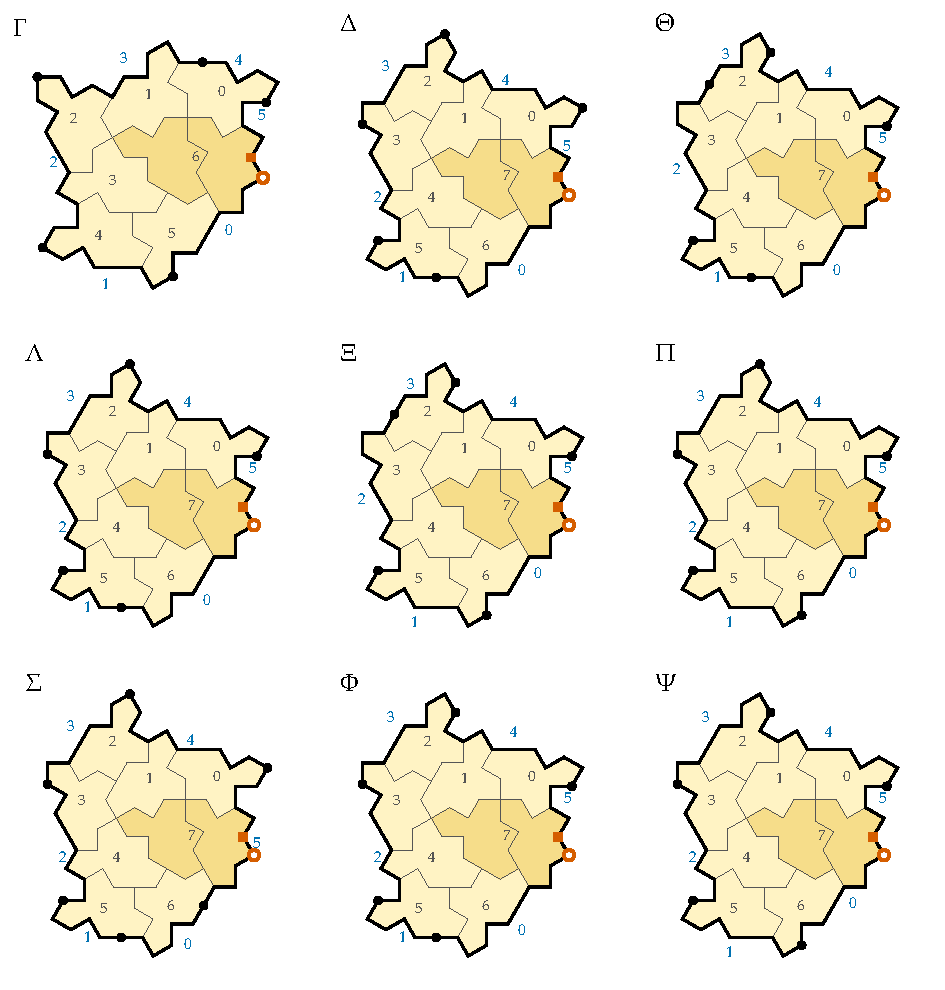
\includegraphics[viewport=#1,clip,width=0.18\textwidth]{figs/level1.pdf}}%
\lone{4.0 330.2 136.0 471.2}\hfill\lone{155.2 330.2 287.2 471.2}\hfill\lone{306.4 330.2 438.4 471.2}\hfill\lone{4.0 171.8 136.0 312.8}\hfill\lone{155.2 171.8 287.2 312.8}\\[2pt]
\hspace*{0.1\textwidth}\lone{306.4 171.8 438.4 312.8}\hfill\lone{4.0 13.4 136.0 154.4}\hfill\lone{155.2 13.4 287.2 154.4}\hfill\lone{306.4 13.4 438.4 154.4}\hspace*{0.1\textwidth}
\caption{The nine level-$1$ supertiles, with tiles of the handedness of $\Tile$ (\cite[Fig.~2.1]{SMKGS-spectre} draws
their mirror images). The Mystic is the darker pair of tiles. Grey numbers: the children (\cref{tab:children}); black
dots: the six vertices; blue numbers: the sides, numbered clockwise (the own orientation at level~$1$); open circle:
the crossover corner $A$, which is vertex~$0$, except for $\Sigma$, where it lies inside side~$5$; filled square: the
corner $B$ (\cref{sec:own}).}
\label{fig:level1}
\end{figure}

The level-$1$ supertiles are the Spectre clusters ($9$ tiles) and the Mystic cluster ($8$ tiles, kind $\Gamma$)
of~\cite[Fig.~2.1]{SMKGS-spectre}, with the markings of~\cite[Fig.~4.1]{SMKGS-spectre}, up to reflection:
\cite[Fig.~2.1]{SMKGS-spectre} draws the clusters with tiles of the opposite handedness to its single Spectre and
Mystic, and so to $\Tile$; \cref{fig:level1} draws them with that of $\Tile$. Explicitly, if the first tile of the
Mystic (child~$7$) is $\Tile$, then child $c\le6$ of a level-$1$ supertile of kind $K\neq\Gamma$ is $f_c(\Tile)$, with
$f_c(z)=\rho^{r_c}z+t_c$, $(r_0,\dots,r_6)=(8,10,10,0,2,2,4)$ and $(t_0,\dots,t_6)=(3+\rho+\rho^3,\allowbreak\
2+\rho+2\rho^2+\rho^3,\allowbreak\ 4+2\rho+\rho^2+2\rho^3,\allowbreak\ 2+2\rho+2\rho^2+2\rho^3,\allowbreak\
1+2\rho+\rho^2+2\rho^3,\allowbreak\ 3\rho^2+3\rho^3,\allowbreak\ 1+\rho^2+3\rho^3)$; the level-$1$ $\Gamma$-supertile is
this cluster without child~$2$, with children $3,\dots,7$ renumbered $2,\dots,6$. In this frame the
crossover corner $A$ (\cref{sec:own}) is $0$, and the six vertices lie where \cref{comp:base} records them: at the
distances from $A$, in own order, that \cref{tab:letters}, $\ell_1$ and $d_1$ give. \Cref{fig:level1} draws the
clusters up to a rotation and a translation.

Combinatorially, the level-$1$ supertiles are the marked hexagons of~\cite[Fig.~4.2]{SMKGS-spectre}, and the level-$n$
supertiles that~\cite[\S5]{SMKGS-spectre} builds from these hexagons are our level-$(n+1)$ supertiles. The edges of
these hexagons carry the labels $x^{+}$, $x^{-}$ ($x\in\{\alpha,\beta,\gamma,\delta,\epsilon,\zeta,\theta\}$) and $\eta$
of~\cite[Fig.~4.2]{SMKGS-spectre} (\cref{tab:letters}); two hexagons sharing an edge carry $x^+$ and $x^-$, or $\eta$
and $\eta$, on it (the \emph{matching rule} of~\cite[\S4]{SMKGS-spectre}). For each kind $T$, the \emph{panel} $T$
of~\cite[Fig.~5.1]{SMKGS-spectre} shows the eight (for $\Gamma$, seven) hexagons, with their kinds, that make up a
hexagon of kind $T$ one level up, with that hexagon's six vertices and the labels of its edges.

The following theorem restates, in our language, results of~\cite{SMKGS-spectre}.

\begin{theorem}[Smith, Myers, Kaplan, Goodman-Strauss~\cite{SMKGS-spectre}]\label{thm:smkgs}
Let $\T$ be a homochiral tiling by $\Tile$.
\begin{enumerate}[label=\textup{(\alph*)}]
\item \textup{\cite[Thms.~2.2, 3.1, 4.1, \S5, Fig.~2.1]{SMKGS-spectre}} The tiles of $\T$ group uniquely into level-$1$
supertiles, each the image under a rotation and a translation of one of the clusters of \cref{fig:level1} (those
of~\cite[Fig.~2.1]{SMKGS-spectre}, reflected). Each contains one Mystic, in the position shown
in~\cite[Fig.~2.1]{SMKGS-spectre}; this Mystic and the other
tiles, taken singly, are the level-$0$ supertiles inside it. For every $m\ge1$ the level-$m$ supertiles of $\T$ group
uniquely into level-$(m+1)$ supertiles. Each tile lies in a unique nested sequence $X_0\subset X_1\subset\cdots$ with
$X_m$ a level-$m$ supertile.
\item \textup{\cite[Thms.~3.1, 4.1, 5.1, \S5, Fig.~4.1]{SMKGS-spectre}} For every $m\ge 1$, the tiling of the plane by the level-$m$
supertiles of $\T$ is combinatorially equivalent (homeomorphic as a topological complex~\cite[\S2.2]{SMKGS-spectre}) to a
tiling by regular hexagons. Each level-$m$ supertile of kind $K$ corresponds to a hexagon marked as the hexagon $K$
of~\cite[Fig.~4.2]{SMKGS-spectre} if $m$ is even, and as its mirror image if $m$ is odd; adjacent supertiles correspond
to hexagons that share an edge, and the labels on that edge match. The grouping into level-$(m+1)$ supertiles
corresponds, up to reflection, to the grouping of hexagons shown in~\cite[Fig.~5.1]{SMKGS-spectre}, and the six points
where a level-$(m+1)$ supertile of kind $T$ meets two others correspond to the six points marked on the outline of the
panel $T$. At level~$1$, the six points where a supertile meets two others correspond to the dots marked on its cluster
in~\cite[Fig.~4.1]{SMKGS-spectre}, the points by which the proof of~\cite[Thm.~4.1]{SMKGS-spectre} tells the clusters
apart.
\end{enumerate}
\end{theorem}

In (a), \cite[Thm.~4.1]{SMKGS-spectre} gives the clusters and~\cite[Thm.~2.2]{SMKGS-spectre} the uniqueness at every
level; we use uniqueness only to speak of \emph{the} hierarchy of $\T$, and, in \cref{sec:nest}, to identify the hierarchy of
the nest tiling. In (b), the choice of mirror image at odd $m$ is
fixed at $m=1$, where our level-$1$ supertiles are the mirror images of the clusters in~\cite[Figs.~2.1,
4.1]{SMKGS-spectre} (see the base case of ($\ast$) in the proof of \cref{prop:pattern}); the choice alternates with $m$
by~\cite[Thm.~5.1]{SMKGS-spectre}.

By \cref{thm:smkgs}(b), every level-$m$ supertile ($m\ge1$) is a closed topological disc whose boundary, its \emph{rim}, is a
simple closed polygon made of tile edges. Its \emph{vertices} are the six points of the rim where it meets two other
level-$m$ supertiles, and its \emph{sides} are the six arcs of the rim between consecutive vertices. (The tile
vertices on a rim are called \emph{rim vertices}; for a supertile of level $\ge1$, ``vertex'' alone always means one of
the six.) If a vertex of one level-$m$ supertile lies on the rim of another, it is a vertex of the other too, since
exactly three level-$m$ supertiles meet there. Each side is shared, as a path of tile edges, with exactly one
neighbouring supertile.

\subsection{Own orientation, side numbering and the crossover corner}\label{sec:own}
By \cref{thm:smkgs}(b), the cyclic order of the labelled sides reverses at each level, so we orient supertiles
alternately; then side $j$ of a supertile of kind $K$ carries the same label at every level (\cref{tab:letters}), and
one composition pattern serves all levels.

\begin{definition}[Own orientation]\label{def:own}
The \emph{own orientation} of a level-$m$ supertile is anticlockwise if $m$ is even and clockwise if $m$ is odd.
We write $\omega_m=(-1)^m$. Its \emph{own order} is the cyclic order in which this orientation runs round its rim.
\end{definition}

Thus a child and its parent are always oriented oppositely. Each supertile of level $m\ge1$ has a distinguished rim
vertex $A$, its \emph{crossover corner}, defined recursively: for a level-$1$ supertile, $A$ is the vertex $v_0$ of the
first tile of its Mystic; for a level-$(m+1)$ supertile, $m\ge1$, $A$ is the crossover corner of its $\Gamma$ child.
(That this point lies on the rim is computed at level $1$ and follows from \cref{prop:pattern}(d) at higher levels.)
The second corner $B$ is the rim vertex next to $A$ anticlockwise (the sense in which $v_1$ follows $v_0$ on
$\Tile$); as own order alternates with $m$, this is $B=A+\omega_m$ in its own order. We call $A$ and $B$ the
\emph{crossover corners}, since the supertile's two crossover arcs run between them (\cref{thm:signature}), as a tile's
two crossover pieces run between $v_0$ and $v_1$ (\cref{def:decoration}). The vertices of a level-$m$ supertile
($m\ge1$) are numbered $0,\dots,5$ in its own order, starting with the first vertex at or after $A$; side $j$ runs from
vertex $j$ to vertex $j+1$ (\cref{fig:level1}).

\subsection{The composition pattern}\label{sec:pattern}
By \cref{thm:smkgs}(b), every level from level~$2$ up is assembled from the one below in the same combinatorial way.
We record this in our numbering.

\begin{definition}[Composition pattern]\label{def:pattern}
The \emph{composition pattern} gives, for each parent kind $T$, the kinds $K_0,\dots,K_{n_T-1}$ of the children
(\cref{tab:children}); for each side of each child, the sibling's side across it, or $\rim$ if it lies on the parent's
rim (\cref{tab:sides}); and for each side of the parent, the children's sides that make it up, in the parent's own order
(\cref{tab:psides}). \Cref{fig:pattern} draws it.
\end{definition}

\begin{figure}[t]
\centering
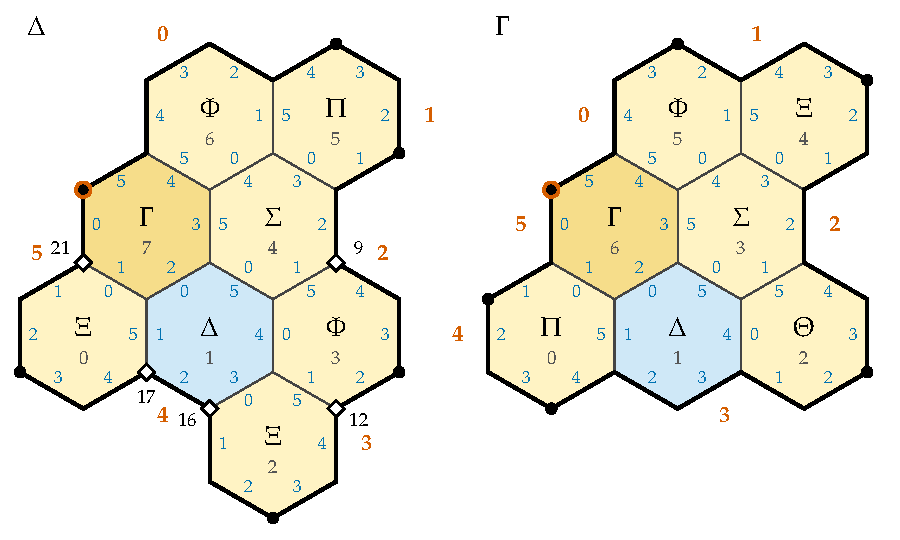
\includegraphics[width=0.66\textwidth]{figs/pattern.pdf}
\caption{The composition pattern for $\Delta$ (left) and for $\Gamma$ (right), in the layout
of~\cite[Fig.~5.1]{SMKGS-spectre}. Each hexagon is a child: kind, number (grey), sides $0$--$5$ (blue); child~$1$, a
$\Delta$, is shaded light blue, and the $\Gamma$ child darker. Thick black: the parent's rim; dots: its vertices;
vermilion: its sides; circled: its crossover corner, vertex~$0$ of the $\Gamma$ child. Left, open diamonds: the
junctions $9,12,16,17,21$ of \cref{sec:junctions}. Every parent kind but $\Gamma$ has the children and gluing of the left
panel, with the kinds of \cref{tab:children}, but its own vertices and side numbers (\cref{tab:psides}). The children's
sides run anticlockwise and the parent's clockwise, their own orientations when the children have even level; for
odd level, take the mirror image.}
\label{fig:pattern}
\end{figure}

\begin{table}[t]
\centering\small
\setlength{\tabcolsep}{3.6pt}
\caption{Adjacency of the children's sides: the entry $c'.j'$ in row $c$, column $j$ means that side $j$ of child $c$
is side $j'$ of child $c'$; $\rim$ means that it lies on the parent's rim.}
\label{tab:sides}
\begin{tabular}[t]{c@{\hspace{1.2em}}cccccc}
\toprule
\multicolumn{7}{c}{every parent kind except $\Gamma$}\\
\midrule
child & side 0 & 1 & 2 & 3 & 4 & 5\\
\midrule
0 & 7.1 & $\rim$ & $\rim$ & $\rim$ & $\rim$ & 1.1\\
1 & 7.2 & 0.5 & $\rim$ & 2.0 & 3.0 & 4.0\\
2 & 1.3 & $\rim$ & $\rim$ & $\rim$ & $\rim$ & 3.1\\
3 & 1.4 & 2.5 & $\rim$ & $\rim$ & $\rim$ & 4.1\\
4 & 1.5 & 3.5 & $\rim$ & 5.0 & 6.0 & 7.3\\
5 & 4.3 & $\rim$ & $\rim$ & $\rim$ & $\rim$ & 6.1\\
6 & 4.4 & 5.5 & $\rim$ & $\rim$ & $\rim$ & 7.4\\
7 & $\rim$ & 0.0 & 1.0 & 4.5 & 6.5 & $\rim$\\
\bottomrule
\end{tabular}\qquad
\begin{tabular}[t]{c@{\hspace{1.2em}}cccccc}
\toprule
\multicolumn{7}{c}{parent kind $\Gamma$}\\
\midrule
child & side 0 & 1 & 2 & 3 & 4 & 5\\
\midrule
0 & 6.1 & $\rim$ & $\rim$ & $\rim$ & $\rim$ & 1.1\\
1 & 6.2 & 0.5 & $\rim$ & $\rim$ & 2.0 & 3.0\\
2 & 1.4 & $\rim$ & $\rim$ & $\rim$ & $\rim$ & 3.1\\
3 & 1.5 & 2.5 & $\rim$ & 4.0 & 5.0 & 6.3\\
4 & 3.3 & $\rim$ & $\rim$ & $\rim$ & $\rim$ & 5.1\\
5 & 3.4 & 4.5 & $\rim$ & $\rim$ & $\rim$ & 6.4\\
6 & $\rim$ & 0.0 & 1.0 & 3.5 & 5.5 & $\rim$\\
\bottomrule
\end{tabular}
\end{table}

\begin{table}[t]
\centering\small
\setlength{\tabcolsep}{3.2pt}
\caption{The parent's sides as concatenations of children's sides. An entry $c.j$ is side $j$ of child $c$, which the
parent's own orientation traverses from vertex $j+1$ to vertex $j$ of the child. Side $J$ of the parent consists of the
entries from its first position up to, but not including, the first position of side $J+1$ (cyclically). For
$T\neq\Sigma$ the parent's side $0$ begins at vertex $0$ of the $\Gamma$ child, which is the parent's crossover corner.
For $T=\Sigma$ the crossover corner lies inside side $5$ (positions $19,20,21,0,1$), after the children's sides $0.2$,
$0.1$, $7.0$.}
\label{tab:psides}
\emph{Eight children} (every $T\neq\Gamma$): the parent's rim, in the parent's own order from vertex $0$ of child $7$.\\[2pt]
\begin{tabular}{l@{\hspace{1em}}*{11}{c}}
\toprule
position & 0 & 1 & 2 & 3 & 4 & 5 & 6 & 7 & 8 & 9 & 10\\
child side & 7.5 & 6.4 & 6.3 & 6.2 & 5.4 & 5.3 & 5.2 & 5.1 & 4.2 & 3.4 & 3.3\\
\midrule
position & 11 & 12 & 13 & 14 & 15 & 16 & 17 & 18 & 19 & 20 & 21\\
child side & 3.2 & 2.4 & 2.3 & 2.2 & 2.1 & 1.2 & 0.4 & 0.3 & 0.2 & 0.1 & 7.0\\
\bottomrule
\end{tabular}

\medskip
\begin{tabular}[t]{l@{\hspace{1em}}*{6}{>{\centering\arraybackslash}p{1.3em}}}
\toprule
parent & \multicolumn{6}{c}{first position of side}\\
& 0 & 1 & 2 & 3 & 4 & 5\\
\midrule
$\Delta$ & 0 & 5 & 7 & 11 & 14 & 19\\
$\Theta$ & 0 & 5 & 7 & 13 & 15 & 20\\
$\Lambda$ & 0 & 5 & 7 & 11 & 14 & 20\\
$\Xi$ & 0 & 3 & 7 & 13 & 15 & 20\\
$\Pi$ & 0 & 3 & 7 & 11 & 14 & 20\\
$\Sigma$ & 2 & 5 & 7 & 11 & 14 & 19\\
$\Phi$ & 0 & 5 & 7 & 11 & 15 & 20\\
$\Psi$ & 0 & 3 & 7 & 11 & 15 & 20\\
\bottomrule
\end{tabular}\qquad
\begin{minipage}[t]{0.56\textwidth}\centering
\emph{Seven children} ($T=\Gamma$), from vertex $0$ of child $6$;\\ sides $0,\dots,5$ begin at positions $0,3,6,11,16,18$.\\[2pt]
\begin{tabular}[t]{l@{\hspace{1em}}*{10}{c}}
\toprule
position & 0 & 1 & 2 & 3 & 4 & 5 & 6 & 7 & 8 & 9\\
child side & 6.5 & 5.4 & 5.3 & 5.2 & 4.4 & 4.3 & 4.2 & 4.1 & 3.2 & 2.4\\
\midrule
position & 10 & 11 & 12 & 13 & 14 & 15 & 16 & 17 & 18 & 19\\
child side & 2.3 & 2.2 & 2.1 & 1.3 & 1.2 & 0.4 & 0.3 & 0.2 & 0.1 & 6.0\\
\bottomrule
\end{tabular}
\end{minipage}
\end{table}

\begin{table}[t]
\centering\small
\caption{The label of~\cite[Fig.~4.2]{SMKGS-spectre} carried by side $j$ of a supertile of each kind: the label of the
edge of the hexagon in direction W, SW, SE, E, NE, NW for $j=0,\dots,5$.}
\label{tab:letters}
\begin{tabular}{c@{\hspace{1.2em}}cccccc}
\toprule
kind & side 0 & side 1 & side 2 & side 3 & side 4 & side 5\\
\midrule
$\Gamma$ & $\alpha^-$ & $\alpha^+$ & $\gamma^-$ & $\delta^-$ & $\beta^+$ & $\beta^-$\\
$\Delta$ & $\gamma^+$ & $\beta^+$ & $\epsilon^-$ & $\alpha^+$ & $\gamma^-$ & $\zeta^-$\\
$\Theta$ & $\gamma^+$ & $\beta^+$ & $\theta^+$ & $\beta^+$ & $\eta$ & $\beta^-$\\
$\Lambda$ & $\gamma^+$ & $\beta^+$ & $\epsilon^-$ & $\alpha^+$ & $\theta^-$ & $\beta^-$\\
$\Xi$ & $\alpha^-$ & $\epsilon^+$ & $\theta^+$ & $\beta^+$ & $\eta$ & $\beta^-$\\
$\Pi$ & $\alpha^-$ & $\epsilon^+$ & $\epsilon^-$ & $\alpha^+$ & $\theta^-$ & $\beta^-$\\
$\Sigma$ & $\zeta^+$ & $\beta^+$ & $\epsilon^-$ & $\alpha^+$ & $\gamma^-$ & $\delta^+$\\
$\Phi$ & $\gamma^+$ & $\beta^+$ & $\epsilon^-$ & $\epsilon^+$ & $\eta$ & $\beta^-$\\
$\Psi$ & $\alpha^-$ & $\epsilon^+$ & $\epsilon^-$ & $\epsilon^+$ & $\eta$ & $\beta^-$\\
\bottomrule
\end{tabular}
\end{table}

\begin{proposition}[The pattern holds at every level]\label{prop:pattern}
Let $\T$ be a homochiral tiling by $\Tile$, let $m\ge1$, and let $Y$ be one of its level-$(m+1)$ supertiles, of kind
$T$, with children $X_0,\dots,X_{n_T-1}$. Then:
\begin{enumerate}[label=\textup{(\alph*)}]
\item $X_c$ has kind $K_c$ (\cref{tab:children});
\item side $j$ of $X_c$ is the same path of tile edges as side $j'$ of $X_{c'}$, traversed in the opposite direction,
whenever \cref{tab:sides} lists $c'.j'$, and it lies on the rim of $Y$ when the table lists $\rim$;
\item side $J$ of $Y$ is the concatenation of the children's sides listed in \cref{tab:psides}, and vertex $J$ of $Y$
is vertex $j+1$ of the child $c$ whose side $c.j$ is listed first for side $J$;
\item the crossover corner $A$ of $Y$ is vertex $0$ of its $\Gamma$ child, which is vertex $0$ of $Y$ if $T\neq\Sigma$, and
lies inside side $5$ of $Y$ if $T=\Sigma$.
\end{enumerate}
\end{proposition}

\begin{proof}
By \cref{thm:smkgs}(b), the level-$m$ supertiles inside $Y$ are combinatorially the hexagons of the panel $T$
of~\cite[Fig.~5.1]{SMKGS-spectre}, with hexagon edges as sides and hexagon vertices as vertices. We use the dictionary
\begin{itemize}[leftmargin=2.2em]
\item[($\ast$)] side $j$ of a level-$m$ supertile of kind $K$ carries the label of the edge of hexagon $K$ in direction
W, SW, SE, E, NE, NW for $j=0,\dots,5$ (\cref{tab:letters}; for odd $m$ the supertile corresponds to the mirror image of
hexagon $K$, and own order, then clockwise, meets its labels in the same order); its crossover corner $A$ is vertex~$0$
if $K\neq\Sigma$; if $K=\Sigma$, $A$ is not a vertex, and lies in the relative interior of side~$5$,
\end{itemize}
and show ($\ast$) by induction on $m$. For $m=1$ it is a comparison of the level-$1$ supertiles, whose vertices and
corner $A$ are marked in \cref{fig:level1}, with~\cite[Fig.~4.1]{SMKGS-spectre}. Drawn with the edges in odd directions
lengthened to $\sqrt3$, which turns the tiles into hats and turtles~\cite[\S3]{SMKGS-spectre}, and in the handedness of
that figure, they coincide with its nine marked clusters: the same outlines, with the vertices at the marked dots. In
each cluster our vertex~$0$ is at the leftmost dot, and, read anticlockwise from it, the sides of cluster $K$ carry
the labels of row~$K$ of \cref{tab:letters}; $A$ is that dot (for $\Sigma$, a point of the NW side, which ends there),
on the light tile of the Mystic. A script checks this against a render of the figure, with the labels transcribed from
the figure (\cref{app:computations}). Suppose ($\ast$) holds for the children of $Y$. The panel names the kind of each inner
hexagon but does not show its edge labels; the matching rule fixes the rotation of each. By \cref{tab:letters}, $\delta$
occurs only on side~$3$ of $\Gamma$ and side~$5$ of $\Sigma$, and $\zeta$ only on side~$5$ of $\Delta$ and side~$0$ of
$\Sigma$. The $\Sigma$ child has one side on the panel's rim, and the two sides next to it face siblings other than the
$\Gamma$ and the $\Delta$ child. Its adjacent sides $5$ and $0$ carry $\delta^+$ and $\zeta^+$, so a sibling facing
side~$5$ is the $\Gamma$ child, and one facing side~$0$ the $\Delta$ child. Hence neither of them is the rim side, as
the other would then be next to it and face some other sibling, and neither is next to the rim side; so they face the
$\Gamma$ and the $\Delta$ child, which fixes the rotations of these three. Every other child meets one of them along a side that the latter
labels $\alpha^+$ or $\gamma^-$, and no kind has two sides labelled $\alpha^-$, or two labelled $\gamma^+$, which fixes
its rotation too (a script confirms that there is no other choice; \cref{app:computations}). With these rotations,
\cref{tab:children,tab:sides,tab:psides} transcribe the panel, including its six marked vertices; this gives (a)--(c).
The crossover corner of $Y$ is that of its $\Gamma$ child, the child's vertex~$0$ by ($\ast$), which \cref{tab:psides}
places at the start of the parent's side~$0$ if $T\neq\Sigma$ and inside side~$5$ if $T=\Sigma$; this is (d). Finally,
with the parent's sides numbered as in \cref{sec:own}, the labels that the panel assigns to them are those of
\cref{tab:letters} for every $T$. So ($\ast$) holds for $Y$, and in particular $A$ lies on the rim.
\end{proof}

\begin{remark}[Computer cross-checks of the pattern]\label{rem:patterncheck}
Since the proof uses \cref{tab:children,tab:sides,tab:psides} as transcriptions of~\cite[Fig.~5.1]{SMKGS-spectre},
they were also checked by computer on actual supertiles (evidence, not used in the proof). The patterns of the actual
compositions $m\to m+1$, $m\le7$, equal the tables (in exact arithmetic for $m\le3$; from level~$5$ on, the vertices are
placed by \cref{prop:pattern}(c), so that part is used rather than tested, though at levels~$5$ and~$6$ they agree with
the vertices observed there); and Kaplan's implementation of
the substitution~\cite{KaplanSpectrePage} gives \cref{tab:children} and, tile for tile up to level~$4$, the same
supertiles as \code{exact.py} (\cref{app:computations}).
\end{remark}

\begin{lemma}[Rigidity]\label{lem:rigid}
Any two level-$m$ supertiles of the same kind, in possibly different homochiral tilings, are related by exactly one
proper motion that maps descendants to descendants with the same numbers (children, their children, and so on, down
to the tiles, and the first tile of a Mystic to the first tile). For $m\ge1$ this motion maps the six vertices, the sides and the corner $A$ of one supertile onto those
of the other.
\end{lemma}

\begin{proof}
Induction on $m$. For $m=0$ this is clear, since a tile and a Mystic have no non-trivial proper symmetry. For $m=1$,
the level-$1$ supertiles are images under proper motions of the clusters of \cref{fig:level1} (\cref{thm:smkgs}(a)),
with their vertices at the points marked in~\cite[Fig.~4.1]{SMKGS-spectre} (\cref{thm:smkgs}(b)), their children
numbered as in
\cref{fig:level1}, and $A$ determined by the Mystic. Let $m\ge1$ and let $Y,Y'$ be level-$(m+1)$ supertiles of kind
$T$. By induction, child $c$ of $Y$ is mapped onto child $c$ of $Y'$ (both of kind $K_c$, by \cref{prop:pattern}(a)),
with its numbered vertices, by a unique proper motion $g_c$. If side $j$ of child $c$ is glued to side $j'$ of child
$c'$, then by \cref{prop:pattern}(b), in $Y$ and in $Y'$, vertices $j$ and $j+1$ of $c$ are vertices $j'+1$ and $j'$
of $c'$; so $g_c$ and $g_{c'}$ agree at two distinct points, and hence are equal. The children's adjacency graph is
connected, so all the $g_c$ are one motion $g$; it maps descendants to
descendants with their numbers and, by \cref{prop:pattern}(c),(d), the vertices, sides and corner $A$ of $Y$ onto those
of $Y'$. A proper motion that maps descendants to descendants maps the first tile of the Mystic at the bottom of the
chain of last ($\Gamma$) children to its counterpart, so it equals $g$, since a tile has no symmetry.
\end{proof}

% ---------------------------------------------------------------------------------------------------------
\section{The decoration and its strands}\label{sec:decoration}

\subsection{Ports and pieces}
Let $t$ be a tile and $e$ one of its edges, with endpoints $x$ and $y$. The tile has two \emph{ports} on $e$, the
port \emph{near $x$} and the port \emph{near $y$}; formally, they are the triples $(t,e,x)$ and $(t,e,y)$. In the
drawing (\cref{fig:tileports}), $e$ carries one crossing point, where two ribbon ends of $t$ meet; followed
from there into $t$, one piece runs towards $x$ and the other towards $y$. These ends are the two ports. For a vertex $v_i$ of $\Tile$, write
\[
\Rp(v_i)=\text{the port on } e_i \text{ near } v_i,\qquad \Lp(v_i)=\text{the port on } e_{i-1} \text{ near } v_i ,
\]
the ports just after and just before the vertex $v_i$ in anticlockwise order. Each of the $28$ ports is
$\Rp(v_i)$ or $\Lp(v_i)$ for exactly one $i$.

\begin{definition}[The decoration]\label{def:decoration}
The \emph{decoration} pairs the $28$ ports of $\Tile$ by fourteen \emph{pieces}:
\[
\underbrace{\Lp(v_i)\leftrightarrow\Rp(v_i)\quad(2\le i\le 13)}_{\text{twelve hooks}},\qquad
\underbrace{\Rp(v_0)\leftrightarrow\Rp(v_1),\qquad \Lp(v_0)\leftrightarrow\Lp(v_1)}_{\text{the crossover}}.
\]
Every tile of a homochiral tiling carries the image of this decoration.
\end{definition}

Each hook turns back round one vertex; the two crossover pieces cross once inside the tile.

\begin{figure}[t]
\centering
\begin{minipage}[c]{0.47\textwidth}\centering
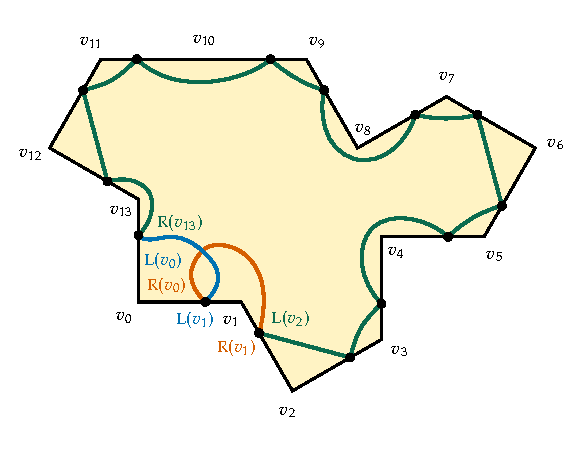
\includegraphics[width=\textwidth]{figs/tileports.pdf}
\end{minipage}\hfill
\begin{minipage}[c]{0.42\textwidth}\centering
\begin{tikzpicture}[scale=0.78,xscale=-1]
\def\n{14}
\fill[tilefill] (0,0) circle (2);
\draw[thick] (0,0) circle (2);
\foreach \k in {0,...,13} {
  \pgfmathsetmacro{\a}{90-360/\n*\k}
  \fill (\a:2) circle (1.3pt);
}
% hooks at k = 2..13 (A = vertex 0 at angle 90, B = vertex 1 at angle 90-360/14 before mirroring);
% mirrored by xscale=-1: rim anticlockwise, B the anticlockwise neighbour of A
\foreach \k in {2,...,13} {
  \pgfmathsetmacro{\a}{90-360/\n*\k}
  \pgfmathsetmacro{\al}{\a+360/\n*0.3}
  \pgfmathsetmacro{\ar}{\a-360/\n*0.3}
  \draw[ribedge,line width=1.1pt] (\al:2) .. controls (\al:1.62) and (\ar:1.62) .. (\ar:2);
}
\pgfmathsetmacro{\aA}{90} \pgfmathsetmacro{\aB}{90-360/14}
\coordinate (RA) at ({\aA-360/14*0.3}:2); \coordinate (LA) at ({\aA+360/14*0.3}:2);
\coordinate (RB) at ({\aB-360/14*0.3}:2); \coordinate (LB) at ({\aB+360/14*0.3}:2);
\draw[oiverm,line width=1.3pt] (RA) .. controls (80:1.0) and (55:1.2) .. (RB);
\draw[oiblue,line width=1.3pt] (LA) .. controls (95:1.2) and (70:1.0) .. (LB);
\node at (90:2.3) {$A$}; \node at ({90-360/14}:2.3) {$B$};
\node[font=\scriptsize,oiblue] at (110:2.95) {$\Lp(A)$};
\node[font=\scriptsize,oiverm] at (89:3.0) {$\Rp(A)$};
\node[font=\scriptsize,oiblue] at (69:3.0) {$\Lp(B)$};
\node[font=\scriptsize,oiverm] at (48:2.95) {$\Rp(B)$};
\end{tikzpicture}
\end{minipage}
\caption{Left: the decoration (centre lines of the ribbons of \cref{fig:tile}). Each edge carries one crossing point
(dot), where two pieces end; on $e_i$ their ends are the ports $\Rp(v_i)$, whose piece runs from the dot towards $v_i$, and
$\Lp(v_{i+1})$, whose piece runs from it towards $v_{i+1}$. Green: the twelve hooks $\Lp(v_i)\leftrightarrow\Rp(v_i)$; vermilion
$\Rp(v_0)\leftrightarrow\Rp(v_1)$ and blue $\Lp(v_0)\leftrightarrow\Lp(v_1)$: the crossover at $A=v_0$, $B=v_1$. Right:
the \emph{signature} at $(A,B)$ (\cref{def:signature}) on a rim of $14$ vertices (dots), oriented anticlockwise as
for the tile: a hook at every rim vertex but $A$ and $B$, and the crossover arcs $\Rp(A)\leftrightarrow\Rp(B)$,
$\Lp(A)\leftrightarrow\Lp(B)$. The tile has it (\cref{lem:tilesig}); so does every supertile of level $m\ge1$, seen as a
black box (\cref{thm:signature}).}
\label{fig:tileports}\label{fig:signature}
\end{figure}

\subsection{The straight-through rule}
Let $\T$ be a homochiral tiling, and let $e=xy$ be an edge shared by tiles $t$ and $t'$.

\begin{definition}[Straight-through rule]\label{def:rule}
The port of $t$ on $e$ near $x$ is \emph{joined} to the port of $t'$ on $e$ near $y$, and the port of $t$ near $y$ to
the port of $t'$ near $x$.
\end{definition}

This is what a ribbon does when it continues straight through the crossing point (\cref{fig:zigzag}, $n=1$). In our
drawing the crossing point of $e_i$ is at distance $0.5+0.15(-1)^i$ from $v_i$. Since $e_i$ of one tile is always
glued, traversed the other way, to some $e_j$ of the other with $i+j$ odd (by the vertex colouring of~\cite[proof of
Lemma~2.1]{SMKGS-spectre}), the two tiles' crossing points on $e$ coincide. Directly: by the turning angles in \cref{sec:tile},
the angle of $\Tile$ at $v_i$ is a multiple of $90^\circ$ for even $i$ and of $120^\circ$ for odd $i$. At a vertex of a
tile, every tile containing it has a vertex there, as tiles meet full edge to full edge, and their angles sum to
$360^\circ$, which multiples of $90^\circ$ and of $120^\circ$, some of each, never do. So the tile vertices at a point
are all even or all odd, and as $v_i$ of one tile is $v_{j+1}$ of the other, $i+j$ is odd. The proofs use only
\cref{def:decoration,def:rule}, so any drawing that realises them may be used (\cref{sec:scope}).

\subsection{Strands}\label{sec:strands}
\begin{definition}[Strand graph]\label{def:strandgraph}
Let $\T$ be a homochiral tiling. The \emph{strand graph} $\G(\T)$ is the multigraph with one vertex for each piece of
each tile and, for each pair of ports joined by the straight-through rule, one edge between the two pieces that end at
these ports. A \emph{strand} is a connected component of $\G(\T)$; a strand is \emph{closed} if it is finite.
\end{definition}

\begin{lemma}\label{lem:degree2}
Every vertex of $\G(\T)$ has degree $2$. Hence every strand is either a finite cycle (a closed strand) or a two-way
infinite path.
\end{lemma}

\begin{proof}
A piece has two ends, each a port of its tile on some edge $e$. Tiles meet full edge to full edge (\cref{sec:spectre}),
so in a tiling of the plane $e$ is an edge of exactly one other tile, and each end is joined to exactly one port, an end
of one of that neighbour's pieces. Hence every vertex has degree exactly $2$; joins always link pieces of different
tiles, so $\G(\T)$ has no self-loops. A connected, locally finite multigraph with all degrees $2$ and no self-loops is a
finite cycle (possibly of length $2$) or a two-way infinite path.
\end{proof}

Equivalently, in a tiling of the plane the pieces and the straight-through rule each pair off the ports of all the
tiles, giving two fixed-point-free involutions; the ports of a strand form an orbit of the group they generate. This
is how the formalisation describes strands.

% ---------------------------------------------------------------------------------------------------------
\section{Boxes and the signature}\label{sec:boxes}

\subsection{Patches and boxes}
A \emph{patch} is a finite set $P$ of tiles of a homochiral tiling whose union is a closed disc with a simple polygonal
boundary, the \emph{rim} $\rim P$. Every supertile of level $\ge1$ is a patch (\cref{thm:smkgs}), and so is a tile.
Every rim edge belongs to exactly one tile of $P$. Every other edge of a tile of $P$ is an \emph{interior edge}, shared
by two tiles of $P$: its relative interior lies inside the disc, so the tile across it is in $P$. Let $E=E(P)$ be the number of rim edges, and number the rim vertices $u_0,\dots,u_{E-1}$ in a
chosen orientation of the rim, indices mod $E$; for a supertile we use its own orientation unless we say otherwise.
For a rim vertex $u_k$ define the \emph{rim ports}
\[
\Rp(u_k)=\text{the port on } u_ku_{k+1} \text{ near } u_k,\qquad \Lp(u_k)=\text{the port on } u_{k-1}u_k \text{ near } u_k,
\]
where the port belongs to the tile of $P$ containing that edge. There are $2E$ rim ports. For a single tile, in its own
(anticlockwise) orientation, these are the ports $\Rp(v_i),\Lp(v_i)$ of \cref{sec:decoration}. Reversing the
orientation exchanges $\Rp$ and $\Lp$ at every rim vertex.

\begin{lemma}[The box of a patch]\label{lem:box}
Start at a rim port of $P$ and follow the pieces of the tiles of $P$, crossing interior edges of $P$ by the
straight-through rule. The path ends at a different rim port. This defines a fixed-point-free involution $\pi_P$ of the
set of rim ports. The pieces of $P$ that are not reached from any rim port form finitely many cycles, the
\emph{closed strands of $P$}.
\end{lemma}

\begin{proof}
The pieces of $P$, joined across interior edges, form a finite graph in which a piece has one neighbour for each of its
ends that is not a rim port. Its components are therefore cycles, and paths (possibly a single piece) with exactly two
free ends, which are distinct rim ports. Every rim port is a free end of exactly one such path, so sending each rim
port to the other free end of its path is a fixed-point-free involution, $\pi_P$.
\end{proof}

We call the paths of \cref{lem:box} the \emph{arcs} of $P$; there are exactly $E$ of them. The rim of $P$ with the
pairing $\pi_P$ is the \emph{box} of $P$. All we need to know about the inside of $P$ is its box and whether $P$ has a
closed strand; the next lemma computes both from smaller patches.

\begin{lemma}[Gluing]\label{lem:gluing}
Let a patch $P$ be the union of patches $P_1,\dots,P_n$ with pairwise disjoint interiors. Then the box of $P$ is
determined by the boxes of the $P_i$ together with the identification of their shared rim edges. More precisely,
$\pi_P$ is computed by alternately applying the $\pi_{P_i}$ and the straight-through rule across shared edges, until a
rim port of $P$ is reached. The closed strands of $P$ are those of the $P_i$ together with the cycles of this
alternation that contain no rim port of $P$.
\end{lemma}

\begin{proof}
Every arc of $P$ (\cref{lem:box}) is a concatenation of arcs of the $P_i$ joined across edges shared by two of the
$P_i$; every closed strand of $P$ is either a closed strand of some $P_i$ or a cyclic concatenation of such arcs. The rim
edges of $P$ are the rim edges of the $P_i$ that are not shared by two of them.
\end{proof}

We use \cref{lem:gluing} in two ways: to define the box of a composition, glued from boxes alone (\cref{sec:comp}), and
to compute the box of a supertile from those of its children. For the first, a \emph{box} is taken abstractly: a
cyclically ordered set of rim vertices $u$, each with two ports $\Lp(u),\Rp(u)$, together with a fixed-point-free
involution $\pi$ of these ports; conditions (i) and (ii) of \cref{def:signature} make sense for any box.

\subsection{The signature}
\begin{definition}[Signature]\label{def:signature}
Let $A$ and $B$ be adjacent rim vertices of a patch $P$. We say that $P$ has the \emph{signature at $(A,B)$} if
\begin{enumerate}[label=(\roman*)]
\item $\pi_P(\Lp(u))=\Rp(u)$ for every rim vertex $u\notin\{A,B\}$ (a \emph{hook} at $u$; we also say that $u$ is a
hook of $P$, and call the arc of $P$ from $\Lp(u)$ to $\Rp(u)$ its \emph{hook arc} at $u$);
\item $\pi_P(\Rp(A))=\Rp(B)$ and $\pi_P(\Lp(A))=\Lp(B)$ (the \emph{crossover});
\item $P$ has no closed strand: the ribbon followed from any port of $P$ reaches the rim.
\end{enumerate}
\end{definition}

The definition is symmetric in $A$ and $B$ and does not depend on the orientation of the rim, since reversing it
exchanges $\Lp$ and $\Rp$. A patch with the signature has $E-2$ hook arcs, one at each rim vertex other than
$A$ and $B$, and two crossover arcs. \Cref{fig:signature} (right) shows the signature.

\begin{lemma}\label{lem:tilesig}
A tile has the signature at $(v_0,v_1)$.
\end{lemma}

\begin{proof}
A tile has no interior edge, so $\pi$ is the pairing of \cref{def:decoration}, and every piece has both ends on the rim.
\end{proof}


% ---------------------------------------------------------------------------------------------------------
\section{The Zigzag Lemma}\label{sec:reduce}
\suppressfloats[t]

In this section a patch $P$ is the union of patches $X_c$ (\emph{children}) with disjoint interiors, each $X_c$ having
the signature at some $(A_c,B_c)$, its \emph{crossover corners}. The children and $P$ are all oriented in the same
rotational sense, so two distinct children traverse a common rim path in opposite directions; $\Rp_c(u),\Lp_c(u)$ are
the rim ports of $X_c$ at $u$ in this orientation. (When $P$ is a supertile and the $X_c$ are its children, the common
orientation is the children's own orientation, which is opposite to the own orientation of $P$ (\cref{def:own}); this
exchanges $\Lp$ and $\Rp$ at the rim vertices of $P$ but does not affect whether $P$ has the signature.) Along a shared
path the ribbon zigzags between two children, and only the parity of the path's length matters (\cref{fig:zigzag}).

\begin{lemma}[Zigzag Lemma]\label{lem:zigzag}
Let $u_0u_1\cdots u_n$ ($n\ge1$) be a path of $n$ edges lying on the rims of two distinct children $X_c$ and $X_{c'}$,
traversed by $X_c$ from $u_0$ to $u_n$. Suppose that none of the interior vertices $u_1,\dots,u_{n-1}$ is a crossover
corner of $X_c$ or of $X_{c'}$. Then alternately applying the straight-through rule across the edges $u_ku_{k+1}$ and
the hooks of $X_c$ and $X_{c'}$ at $u_1,\dots,u_{n-1}$ connects the ports of $X_c$ and $X_{c'}$ near $u_0$ on $u_0u_1$
and near $u_n$ on $u_{n-1}u_n$ in pairs as follows:
\begin{align*}
n \text{ even:}\quad & \Rp_c(u_0)\leftrightarrow \Lp_c(u_n), && \Lp_{c'}(u_0)\leftrightarrow \Rp_{c'}(u_n);\\
n \text{ odd:}\quad & \Rp_c(u_0)\leftrightarrow \Rp_{c'}(u_n), && \Lp_{c'}(u_0)\leftrightarrow \Lp_c(u_n).
\end{align*}
These two connections use every port on the edges of the path.
\end{lemma}

For $n=1$ the lemma is the straight-through rule (\cref{def:rule}) written in rim ports; \cref{lem:lengthen,lem:junctionmap}
use it for $n=1$ and $n=3$.

\begin{figure}[t]
\centering
\newcommand{\zz}[3]{% #1 = n, #2 = x offset, #3 = label
\begin{scope}[xshift=#2cm]
\fill[tilefill] (0,0) rectangle (#1,0.75); \fill[tilefill!65!white] (0,0) rectangle (#1,-0.75);
\draw[thick] (0,0)--(#1,0);
\foreach \k in {0,...,#1} { \fill (\k,0) circle (1.2pt); }
\node[font=\scriptsize] at (0,-0.95) {$u_0$}; \node[font=\scriptsize] at (#1,-0.95) {$u_{#1}$};
\draw[oiorange,line width=1.3pt] (0,0.36) \foreach \k in {1,...,#1} { cos ({\k-0.5},0) sin (\k,{0.36*(-1)^\k}) };
\draw[oiblue,line width=1.3pt] (0,-0.36) \foreach \k in {1,...,#1} { cos ({\k-0.5},0) sin (\k,{-0.36*(-1)^\k}) };
\node[font=\small] at ({#1/2},1.0) {#3};
\end{scope}}
\begin{tikzpicture}[scale=0.72]
\node[font=\small] at (-0.55,0.4) {$X_c$}; \node[font=\small] at (-0.55,-0.4) {$X_{c'}$};
\zz{1}{0}{$n=1$}
\zz{3}{1.8}{$n=3$}
\zz{2}{6.1}{$n=2$}
\zz{4}{8.9}{$n=4$}
\end{tikzpicture}
\caption{The Zigzag Lemma. Along a shared path whose interior vertices are hooks of both children, the ribbons cross the
path at every edge and turn back at every interior vertex, alternately in $X_c$ (above) and $X_{c'}$ (below). The orange
connection starts at $\Rp_c(u_0)$ (top left) and the blue one at $\Lp_{c'}(u_0)$ (bottom left). For odd $n$ they end in
the other child, at $\Rp_{c'}(u_n)$ (bottom right) and $\Lp_c(u_n)$ (top right); for even $n$ they end in the child they
started from, at $\Lp_c(u_n)$ and $\Rp_{c'}(u_n)$. Only the parity of $n$ matters, so lengthening a shared path by two
edges changes nothing (\cref{lem:lengthen}).}
\label{fig:zigzag}
\end{figure}

\begin{proof}
Start at $\Rp_c(u_0)$, the port of $X_c$ on $u_0u_1$ near $u_0$ (orange in \cref{fig:zigzag}). The straight-through
rule takes it to the port of $X_{c'}$ on $u_0u_1$ near $u_1$. In the orientation of $X_{c'}$, which runs from $u_1$ to
$u_0$ along this edge, that port is $\Rp_{c'}(u_1)$. If $n=1$ we have reached $\Rp_{c'}(u_n)$. Otherwise $u_1$ is a hook
of $X_{c'}$, which leads to $\Lp_{c'}(u_1)$, the port of $X_{c'}$ on $u_1u_2$ near $u_1$. Crossing $u_1u_2$ leads to the
port of $X_c$ on $u_1u_2$ near $u_2$, which is $\Lp_c(u_2)$. If $n=2$ we stop. Otherwise the hook of $X_c$ at $u_2$ leads
to $\Rp_c(u_2)$, and the pattern repeats with all indices shifted by two. So this connection visits the hooks of
$X_{c'}$ at odd $k$ and those of $X_c$ at even $k$, and ends at $\Lp_c(u_n)$ if $n$ is even and at $\Rp_{c'}(u_n)$ if
$n$ is odd. The second connection starts at $\Lp_{c'}(u_0)$, the port of $X_{c'}$ on $u_0u_1$ near $u_0$. By the same
argument with $X_c,X_{c'}$ exchanged and $\Lp,\Rp$ exchanged, it passes $\Lp_c(u_1)$, $\Rp_c(u_1)$, $\Rp_{c'}(u_2)$,
$\Lp_{c'}(u_2)$, \dots, visits the hooks of $X_c$ at odd $k$ and those of $X_{c'}$ at even $k$, and ends at
$\Rp_{c'}(u_n)$ if $n$ is even and at $\Lp_c(u_n)$ if $n$ is odd. Each connection crosses each of the $n$ edges once,
using two of its four ports, and the two connections use different ports, so together they use all of them.
\end{proof}

% ---------------------------------------------------------------------------------------------------------
\section{Side lengths}\label{sec:lengths}

By the Zigzag Lemma, two boxes glued along a path with hooks at its interior vertices interact only through the parity
of its length. This section shows that the side lengths of the supertiles are given by Fibonacci numbers
(\cref{prop:fib}), so that they grow with the level, and never change parity (\cref{cor:parity}); it also places the crossover
corner (\cref{lem:Apos}). \Cref{sec:induction} uses these facts to reduce every level to level~$1$.

For $m\ge1$, write $\ell_m(K,j)$ for the number of edges of side $j$ of a level-$m$ supertile of kind $K$; by
\cref{lem:rigid} it is well defined.

\subsection{Letters}
By ($\ast$) in the proof of \cref{prop:pattern}, every side of a level-$m$ supertile ($m\ge1$) carries the edge label
of~\cite[Fig.~4.2]{SMKGS-spectre} that \cref{tab:letters} lists. The \emph{letter} of a side is its label without the
sign; there are eight letters, $\alpha,\beta,\gamma,\delta,\epsilon,\zeta,\eta,\theta$. By the matching rule
(\cref{sec:supertiles}), two sides glued to each other have the same letter; for sides glued inside a supertile this
can also be read off \cref{tab:children,tab:sides,tab:letters}.

\begin{proposition}[Lengths by letter]\label{prop:letters}
For every $m\ge1$ the length $\ell_m(K,j)$ depends only on the letter of side $j$ of $K$. Write $x_m$ for the common
length of the level-$m$ sides with letter $x$. Then
\begin{equation}\label{eq:rec}
\begin{aligned}
\alpha_{m+1}&=\beta_m+\epsilon_m+\eta_m, &\qquad \beta_{m+1}&=\alpha_m+\epsilon_m,\\
\gamma_{m+1}&=\beta_m+2\epsilon_m+\eta_m+\theta_m, & \delta_{m+1}&=\alpha_m+\beta_m+\epsilon_m+2\theta_m,\\
\epsilon_{m+1}&=3\epsilon_m+\eta_m, & \zeta_{m+1}&=\alpha_m+\epsilon_m+\theta_m,\\
\eta_{m+1}&=4\epsilon_m+\eta_m, & \theta_{m+1}&=4\epsilon_m+\eta_m+\theta_m,
\end{aligned}
\end{equation}
with $(\alpha_1,\beta_1,\gamma_1,\delta_1,\epsilon_1,\zeta_1,\eta_1,\theta_1)=(7,5,10,10,8,6,10,11)$.
\end{proposition}

\begin{proof}
For $m=1$ this is a direct count on the level-$1$ supertiles (\cref{fig:level1}), recorded in \cref{comp:base}. By
\cref{prop:pattern}(c), $\ell_{m+1}(T,J)$ is the sum of the lengths of the children's sides listed in
\cref{tab:psides}. Inspection of the $54$ parent sides in \cref{tab:children,tab:psides,tab:letters} (also checked by a
script; \cref{app:computations}) shows that the multiset of letters of these children's sides depends only on the
letter of side $J$ of $T$, and is the one in~\eqref{eq:rec}. For example, side $0$ of
$\Delta$ (letter $\gamma$) is made of $7.5,6.4,6.3,6.2,5.4$, with letters $\beta,\eta,\epsilon,\epsilon,\theta$. The
claim follows by induction on $m$.
\end{proof}

The recurrence~\eqref{eq:rec} has a closed form. Let $\Fib_n$ be the Fibonacci numbers, $\Fib_1=\Fib_2=1$.

\begin{proposition}[Fibonacci side lengths]\label{prop:fib}
For every $m\ge1$,
\begin{gather*}
\alpha_m=\Fib_{3m+2}+2,\qquad \beta_m=\Fib_{3m+1}+2,\qquad \gamma_m=\delta_m=\eta_m=2\Fib_{3m+2},\\
\epsilon_m=\Fib_{3m+3},\qquad \zeta_m=2\Fib_{3m+1},\qquad \theta_m=\Fib_{3m+4}-2 .
\end{gather*}
\end{proposition}

\begin{proof}
For $m=1$, $(\Fib_4,\Fib_5,\Fib_6,\Fib_7)=(3,5,8,13)$ gives the initial values. For the induction step put
$a=\Fib_{3m+1}$ and $b=\Fib_{3m+2}$, so that $\Fib_{3m+3}=a+b$, $\Fib_{3m+4}=a+2b$, $\Fib_{3m+5}=2a+3b$,
$\Fib_{3m+6}=3a+5b$ and $\Fib_{3m+7}=5a+8b$. By the induction hypothesis, $\alpha_m=b+2$, $\beta_m=a+2$,
$\gamma_m=\delta_m=\eta_m=2b$, $\epsilon_m=a+b$, $\zeta_m=2a$ and $\theta_m=a+2b-2$. Substituting into~\eqref{eq:rec}:
\begin{gather*}
\alpha_{m+1}=(a+2)+(a+b)+2b=\Fib_{3m+5}+2,\qquad \beta_{m+1}=(b+2)+(a+b)=\Fib_{3m+4}+2,\\
\gamma_{m+1}=(a+2)+2(a+b)+2b+(a+2b-2)=4a+6b=2\Fib_{3m+5},\\
\delta_{m+1}=(b+2)+(a+2)+(a+b)+2(a+2b-2)=4a+6b=2\Fib_{3m+5},\\ \eta_{m+1}=4(a+b)+2b=4a+6b=2\Fib_{3m+5},\qquad
\epsilon_{m+1}=3(a+b)+2b=\Fib_{3m+6},\\ \zeta_{m+1}=(b+2)+(a+b)+(a+2b-2)=2\Fib_{3m+4},\\
\theta_{m+1}=4(a+b)+2b+(a+2b-2)=5a+8b-2=\Fib_{3m+7}-2.\qedhere
\end{gather*}
\end{proof}

Since $\Fib_n$ is even exactly when $3\mid n$ (the parities of $\Fib_1,\Fib_2,\dots$ run odd, odd, even, and
repeat), \cref{prop:fib} gives:

\begin{corollary}[Parities are constant]\label{cor:parity}
For every $m\ge1$ the lengths $\alpha_m$, $\beta_m$, $\theta_m$ are odd and $\gamma_m$, $\delta_m$, $\epsilon_m$,
$\zeta_m$, $\eta_m$ are even.
\end{corollary}

\subsection{The crossover corner}
\begin{lemma}[Position of $A$]\label{lem:Apos}
Let $m\ge1$. For $K\neq\Sigma$, the crossover corner $A$ of a level-$m$ $K$-supertile is its vertex $0$. For
$K=\Sigma$, $A$ lies inside side $5$ (letter $\delta$), $d_m$ edges along it from vertex $5$ and
$\delta_m-d_m=2\Fib_{3m}$ edges from vertex $0$, where
\[
d_m=2\Fib_{3m+1}.
\]
\end{lemma}

\begin{proof}
For $m=1$ the lemma is part of \cref{comp:base}: $A$ is vertex~$0$ if $K\neq\Sigma$, and $d_1=6=2\Fib_4$. For
$m\ge2$ and $K\neq\Sigma$ it is \cref{prop:pattern}(d). For $K=\Sigma$: by \cref{tab:psides}, which lists the
children's sides in the parent's own order, side~$5$ of a level-$(m+1)$ $\Sigma$-supertile begins, at its vertex~$5$,
with the children's sides $0.2$, $0.1$, $7.0$, and by \cref{prop:pattern}(d) its crossover corner comes right after
them.
Child~$0$ is a $\Xi$ and child~$7$ a $\Gamma$, so these sides have letters $\theta,\epsilon,\alpha$, and by
\cref{prop:fib}
$d_{m+1}=\theta_m+\epsilon_m+\alpha_m=(\Fib_{3m+4}-2)+\Fib_{3m+3}+(\Fib_{3m+2}+2)=2\Fib_{3m+4}$. Finally,
$\delta_m-d_m=2\Fib_{3m+2}-2\Fib_{3m+1}=2\Fib_{3m}$ by \cref{prop:fib}.
\end{proof}

\begin{lemma}[Lower bounds]\label{lem:bounds}
For every $m\ge1$: every side has length at least $5$; $d_m\ge6$; and $\delta_m-d_m\ge4$.
\end{lemma}

\begin{proof}
By \cref{prop:fib} all letter lengths increase with $m$, and at $m=1$ the smallest is $\beta_1=5$. Also $d_m\ge d_1=6$ and
$\delta_m-d_m=2\Fib_{3m}\ge 2\Fib_3=4$.
\end{proof}

% ---------------------------------------------------------------------------------------------------------
\section{The signature at every level}\label{sec:induction}

We prove the Signature Theorem by induction on the level, reducing every step to a finite computation at level~$1$,
and deduce \cref{thm:A} from it (\cref{sec:noclosed}).

\subsection{Compositions as a function of side lengths}\label{sec:comp}
A box with the signature at $(A,B)$ is determined by its rim and the places of $A$ and $B$. So, once the children of a
supertile have the signature, the box of the supertile depends, as we show below, only on the tables, the children's
side lengths, the sign that places each $B_c$ next to $A_c$, and the place of the corner $A_\Sigma$ of the $\Sigma$ child,
the one child whose corner $A$ is not a vertex (\cref{lem:Apos}); $d$ below records where on its side~$5$ it lies.

\emph{Compositions.} Fix a parent kind $T$, with children $c=0,\dots,n_T-1$ of kinds $K_c$ (\cref{tab:children}),
exactly one of which, $c_\Sigma$, is a $\Sigma$, and exactly one, the last, a $\Gamma$. Let $L$ assign to each child $c$
and side $j\in\{0,\dots,5\}$ a positive integer $L(c,j)$, with equal values on sides glued by \cref{tab:sides}; let $d$
be an integer with $2\le d\le L(c_\Sigma,5)-2$; and let $\omega\in\{\pm1\}$. The \emph{composition} $C_T(L,d,\omega)$
is the following abstract patch of boxes. Child $c$ has $E_c=\sum_jL(c,j)$ rim vertices, numbered $0,\dots,E_c-1$ in
its own order; its vertex $j$ (one of the six) is rim vertex $V_c(j)=\sum_{i<j}L(c,i)$, and side $j$ runs from
$V_c(j)$ to $V_c(j+1)$. Its crossover corner $A_c$ is rim vertex $0$, or, for $c=c_\Sigma$, rim vertex $V_c(5)+d$, at
distance $d$ from vertex $5$ along side $5$; $B_c=A_c+\omega$ (as $2\le d\le L(c_\Sigma,5)-2$, the corners
$A_\Sigma=A_{c_\Sigma}$ and $B_{c_\Sigma}$ lie strictly inside side~$5$); and it is a box satisfying (i) and (ii) of
\cref{def:signature} at $(A_c,B_c)$. Sides are glued in pairs as in \cref{tab:sides}, reversing direction: the $r$-th
edge of side $j$ of $c$ is the $r$-th edge from the end of side $j'$ of $c'$. The sides marked $\rim$ form the rim of
the composition, in the order of \cref{tab:psides} reversed (the table follows the parent's own orientation; the
composition, like its children, has the opposite one); the ports of a rim vertex are those of the children on its two
rim edges. Following ribbons alternately through a child, by its pairing, and straight across a glued edge, as in
\cref{lem:gluing}, defines the box of the composition and its \emph{closed strands}, the cycles of this alternation
that contain no rim port of the composition. The Zigzag Lemma and its proof apply unchanged to compositions, since they
use only the pairings of the children and the straight-through rule. We say that $C_T(L,d,\omega)$ \emph{has the
signature} if the crossover corners $A_\Gamma,B_\Gamma$ of its $\Gamma$ child are adjacent rim vertices of the
composition and it has the signature at $(A_\Gamma,B_\Gamma)$ (\cref{def:signature}, applied to its box and its closed
strands).

Write $\ell_m$ also for the function $(c,j)\mapsto\ell_m(K_c,j)$; by \cref{sec:lengths} and \cref{lem:bounds},
$C_T(\ell_m,d_m,\omega)$ is defined.

\begin{reduction}[A supertile is its composition]
Let $m\ge1$, and let $Y$ be a level-$(m+1)$ supertile of kind $T$ whose children $X_c$ have the signature at
$(A_c,A_c+\omega_m)$ in their own orientation. Then the children of $Y$, with their rims, sides, corners $A_c,B_c$ and
the gluing of their sides, and the rim of $Y$ read in the children's order, match those of
$C_T(\ell_m,d_m,\omega_m)$. So the box of $Y$ is the box of the composition, and $Y$ has a closed strand if and only if
the composition has one.
\end{reduction}

Indeed: (i)~by \cref{prop:pattern}(a),(b) and \cref{prop:letters} the children have the kinds and side lengths of the
composition, and side $j$ of $X_c$ is side $j'$ of $X_{c'}$ traversed oppositely; (ii)~two children meet only along the
closed sides they share: at a point inside a side of a child, the rim edges there are shared with the partner across
that side, so the child and its partner fill a neighbourhood; and at a vertex exactly three level-$m$ supertiles meet,
any two of them sharing a side that ends there (\cref{thm:smkgs}(b)); (iii)~so each side of a child is wholly shared
with one sibling or wholly on the rim, as in \cref{tab:sides}; (iv)~$A_c$ is placed by \cref{lem:Apos}, and
$B_c=A_c+\omega_m$ by hypothesis; (v)~the rim of the parent is given by \cref{tab:psides} (\cref{prop:pattern}(c)). By
\cref{lem:gluing}, the strands of the supertile are then those of the composition, and its box is the box of
$C_T(\ell_m,d_m,\omega_m)$. Step~(ii) is the one geometric step, argued here: it
ensures that the children touch only along the gluings of (i), so that no other edges join their ribbons. With
\cref{thm:smkgs}, \cref{prop:pattern} and \cref{lem:rigid} it makes up part~(M1) of the link with actual tilings, which the formalisation
does not prove but takes as given (\cref{app:ai}). The compositions themselves are built from the tables alone, and the
tables are consistent: \cref{tab:psides} lists exactly once each side that \cref{tab:sides} puts on the rim, and turning
about the end vertex of each entry, across sides that \cref{tab:sides} glues, leads to the start of the next entry (a
finite check, made in the formalisation). For instance, $7.5$ ends at vertex~$5$ of child~$7$; side~$4$ of child~$7$ is
side~$5$ of child~$6$, so this is vertex~$5$ of child~$6$, whose side~$4$ lies on the rim and is the next entry, $6.4$.

\subsection{Lengthening}\label{sec:lengthen}
Let $(L,d)$ be as above. A \emph{move} lengthens one side of one child by two edges, together with the side glued to it
if there is one. In the composition, an edge $e$ of that side is replaced by a path of three edges through two new
vertices; $e$ must be neither the first nor the last edge of its side (in each child that contains it), nor one of the
two edges at $A_\Sigma$. This ensures that the edge between $A_c$ and $B_c$ is never cut, as the proof of
\cref{lem:lengthen} needs: for a child other than the $\Sigma$ child, $A_c$ is vertex~$0$, the end of side~$5$ and the
start of side~$0$, and $B_c$ is next to it. The result is $(L',d')$: $L'$ is $L$ with the side,
and its partner, two edges longer; $d'=d+2$ if $e$ lies on side $5$ of the $\Sigma$ child between its vertex~$5$ and
$A_\Sigma$, and $d'=d$ otherwise.

\begin{lemma}[Lengthening]\label{lem:lengthen}
If $C_T(L,d,\omega)$ has the signature, then so does $C_T(L',d',\omega)$, for every move $(L,d)\to(L',d')$.
\end{lemma}

\begin{proof}
The idea: on a shared edge, cutting $e$ replaces one crossing by a zigzag along three edges, which joins the same
ports (\cref{lem:zigzag}); on the rim it adds two hooks. Write $C=C_T(L,d,\omega)$ and $C'=C_T(L',d',\omega)$, and
let $e=u_0u_1$. Then $C'$ is $C$ with $e$ cut into three: in each child that contains it, $e$ is replaced by the path
$u_0w_1w_2u_1$, and every vertex of $C$ has an image vertex in $C'$ (the numbers of the rim vertices after $e$ go up
by two). This is only a relabelling: the side and its partner gain the two new edges, every other side keeps its
length, and the $r$-th edge of a side is still glued to the $r$-th from the end of its partner. The conditions on $e$ make the crossover corners of $C'$ the images of those of $C$: for $A_\Sigma$ by the
choice of $d'$, and $B_c=A_c\pm1$ stays next to $A_c$ because the edge between them (the first edge of side $0$, the
last of side $5$, or an edge at $A_\Sigma$) is never cut. In particular $w_1$ and $w_2$ are not crossover corners. Let
$\varphi$ map each port of $C$ to the port of $C'$ of the same child and the same hand ($\Rp$ or $\Lp$) at the image
vertex. Then $\varphi$ commutes with the pairings inside the children, since the crossover corners correspond, and with
the straight-through rule across every glued edge other than $e$. If $e$ is shared by children $c$ and $c'$, with $c$
traversing it from $u_0$ to $u_1$, crossing it joins $\Rp_c(u_0)$ to $\Rp_{c'}(u_1)$ and $\Lp_c(u_1)$ to
$\Lp_{c'}(u_0)$ (\cref{lem:zigzag} with $n=1$); in $C'$, by \cref{lem:zigzag} with $n=3$, the ribbons run along the
new path from $\varphi(\Rp_c(u_0))$ to $\varphi(\Rp_{c'}(u_1))$ and from $\varphi(\Lp_c(u_1))$ to
$\varphi(\Lp_{c'}(u_0))$. If $e$ lies on the rim, $w_1$ and $w_2$ are new rim vertices of $C'$, and hooks of the child,
so hooks of $C'$.

Hence, by induction along the ribbon (each of its steps in $C$, through a child or across a glued edge, is matched in
$C'$, across $e$ by the path along $u_0w_1w_2u_1$), for every port $x$ of $C$, the ribbon of $C'$ from $\varphi(x)$
passes through the images of the ports that the ribbon of $C$ from $x$ meets, and reaches the rim at the image of the rim port reached in $C$. So $C'$ has a hook at
the image of every rim vertex of $C$ other than $A_\Gamma$ and $B_\Gamma$, and at each new rim vertex. As before,
$A_\Gamma$ and $B_\Gamma$ are adjacent; they are still rim vertices, since the rim edges of the $\Gamma$ child at them
stay on the rim, and they carry the crossover. Finally, $C'$ has no closed strand. Every port of $C'$ at the image of
a vertex of $C$ is some $\varphi(x)$, whose ribbon reaches the rim. A port at $w_1$ or $w_2$ lies on the hook there if
$e$ is on the rim, and otherwise on one of the two connections of \cref{lem:zigzag} along $u_0w_1w_2u_1$; these use
every port on these edges and end at ports at $u_0$ and $u_1$, so its ribbon too reaches the rim.
\end{proof}

Call $(L,d)$ \emph{admissible} if sides glued by \cref{tab:sides} have the same
length; $L(c,j)\ge\ell_1(c,j)$ and $L(c,j)\equiv\ell_1(c,j)\pmod2$ for all $c$ and $j$; $d\ge d_1$ and $d\equiv
d_1\pmod2$; and $L(c_\Sigma,5)-d\ge\ell_1(c_\Sigma,5)-d_1=4$. Then $d\ge6$ and $L(c_\Sigma,5)-d\ge4$, so the composition
$C_T(L,d,\omega)$ is defined. Every admissible pair is reached from $(\ell_1,d_1)$ by moves (\cref{lem:reach}), which
only lengthen sides, two edges at a time. Admissible pairs need not be the side lengths of actual supertiles, since $L$
may give different lengths to sides with the same letter.

\begin{lemma}[Reachability]\label{lem:reach}
\textup{(a)} For every $m\ge1$, the pair $(\ell_m,d_m)$ is admissible. \textup{(b)} Every admissible
$(L,d)\neq(\ell_1,d_1)$ arises by a move from an admissible pair $(\bar L,\bar d)$ with
$\sum_{c,j}\bar L(c,j)<\sum_{c,j}L(c,j)$. The move can be chosen so that its edge $e$ lies at least two edges from both
ends of its side (at least two edges of the side precede $e$ and at least two follow it), in each child that contains
it, unless that side is side $5$ of the $\Sigma$ child or is glued to it. (This is used only for the junction map of
\cref{sec:junctions}.)

Hence a property of pairs that holds at $(\ell_1,d_1)$ and is kept by the moves of \textup{(b)} holds at every
admissible pair, in particular at $(\ell_m,d_m)$ for every $m\ge1$.
\end{lemma}

\begin{proof}
(a) Glued sides have the same letter (\cref{sec:lengths}), so by \cref{prop:letters} the same length. By
\cref{prop:fib} the letter lengths do not decrease with $m$, and by \cref{cor:parity} their parities do not change. By
\cref{lem:Apos}, $d_m=2\Fib_{3m+1}$ is even, and by \cref{lem:bounds}, $d_m\ge6=d_1$ and
$\ell_m(c_\Sigma,5)-d_m=\delta_m-d_m\ge4$.

(b) If $L=\ell_1$, then $L(c_\Sigma,5)=\delta_1=10$ and $d_1\le d\le 10-4=d_1$, so $(L,d)=(\ell_1,d_1)$, which is
excluded. Hence $L\neq\ell_1$, and by the parity condition some side $j$ of some child $c$ has
$L(c,j)\ge\ell_1(c,j)+2$; we undo a move on that side. If the side is neither side $5$ of the $\Sigma$ child nor glued
to it, take $\bar d=d$ and the move whose edge is the third edge of the side (the third from the end in the partner):
before the move the side has length at least $\ell_1(c,j)\ge5$ (\cref{lem:bounds}), so this edge lies at least two
edges from both ends, in either child. Otherwise, measure distances along side $5$ of the $\Sigma$ child from its
vertex $5$. If $d\ge d_1+2$, take $\bar d=d-2$ and the move whose edge is the second edge of the side, before
$A_\Sigma$; it does not touch $A_\Sigma$, since $\bar d\ge6$. If $d=d_1$, take $\bar d=d$ and the move whose edge is the
second edge after $A_\Sigma$: since $L(c_\Sigma,5)\ge\ell_1(c_\Sigma,5)+2$ by the choice of the side, before the move
it has $L(c_\Sigma,5)-2-d\ge\ell_1(c_\Sigma,5)-d_1=4$ edges after $A_\Sigma$, so this edge is at least two edges from
the end of the side. In each case $(\bar L,\bar d)$ is admissible: the side, and the side glued to it if there is one, are two edges
shorter, so still equal, at least $\ell_1$ and of its parity, as $L(c,j)\ge\ell_1(c,j)+2$; $\bar d\ge d_1$ and
$\bar d\equiv d_1\pmod2$; and $\bar L(c_\Sigma,5)-\bar d$ is $L(c_\Sigma,5)-d\ge4$ in the first two cases and at least $4$
in the third, as shown. And $\sum\bar L=\sum L-2$ or $\sum L-4$. The final
assertion of the lemma follows by induction on $\sum_{c,j}L(c,j)$.
\end{proof}

\begin{computation}[The compositions at the level-$1$ lengths]\label{comp:compose}
For each of the nine kinds $T$ and both signs $\omega$, the composition $C_T(\ell_1,d_1,\omega)$ has the signature.
\end{computation}

This was computed by \code{hierarchy/compositions.py}, which builds the $18$ compositions from
\cref{tab:children,tab:sides,tab:psides,tab:letters} and $\ell_1$, $d_1$ alone and follows the ribbon from every port;
the Lean kernel repeats it (\cref{app:computations}). Both signs are needed, although a level-$2$ supertile is glued as
$C_T(\ell_1,d_1,\omega_1)$ with $\omega_1=-1$ (\cref{sec:comp}): moves keep $\omega$, whereas the sign $\omega_m$ used
at level $m+1$ alternates with $m$.

Most of the signature of a composition is automatic. Only the $\Gamma$ child has its crossover corners on the rim: its
sides $5$ and $0$, which meet at $A_\Gamma$, lie on the rim (\cref{tab:sides}), while the crossover corners of every
other child lie on sides it shares with siblings, away from the rim. So $A_\Gamma,B_\Gamma$ carry the crossover of the
$\Gamma$ child, and every other rim vertex whose two rim edges belong to one child is a hook of that child. The
computation decides the rest: the hooks at the eight rim vertices (seven for $T=\Gamma$) where the rim passes from one
child to another, and that no strand closes.

\begin{proposition}[Compositions at every level]\label{prop:compose}
For every $m\ge1$, every kind $T$ and both signs $\omega$, the composition $C_T(\ell_m,d_m,\omega)$ has the signature.
\end{proposition}

\begin{proof}
Fix $T$ and $\omega$, and consider the property of $(L,d)$ that $C_T(L,d,\omega)$ has the signature. It holds at
$(\ell_1,d_1)$ by \cref{comp:compose}, and every move keeps it by \cref{lem:lengthen}; so by \cref{lem:reach} it holds
at $(\ell_m,d_m)$.
\end{proof}

\subsection{The induction}\label{sec:induct}
\begin{computation}[Base case]\label{comp:base}
Each of the nine level-$1$ supertiles of \cref{fig:level1}, and so by \cref{lem:rigid} every level-$1$ supertile, has
the side lengths $\ell_1(K,j)=x_1$, where $x$ is the letter of side $j$ (\cref{tab:letters}) and
$(\alpha_1,\dots,\theta_1)=(7,5,10,10,8,6,10,11)$; its crossover corner $A$ is vertex~$0$ if its kind is not $\Sigma$,
and for $\Sigma$ lies inside side~$5$, $d_1=6$ edges along it from vertex~$5$; and it has the signature at $(A,B)$,
where $B=A+\omega_1$ in its own order.
\end{computation}

This was computed from the tiles in exact arithmetic by the program \code{exact/exact.py}, which uses \cref{lem:gluing}
and checks each clause of the statement on the nine supertiles; \code{hierarchy/checks.js} checks the signature again
in floating point. The kernel of
Lean repeats the check on the nine level-$1$ supertiles computed by \code{exact.py}, taken as input, so it checks
neither their geometry nor that $A$ is $v_0$ of the first tile of its Mystic (\cref{app:computations,app:ai}). The
induction starts here, not at the tile (\cref{lem:tilesig}), because the composition pattern describes level $m+1$
from level $m\ge1$ only; level $1$ is assembled from tiles and a Mystic.

\begin{theorem}[Signature Theorem]\label{thm:signature}
In every homochiral tiling by $\Tile$, for every $m\ge1$, every level-$m$ supertile of every kind has the signature at
$(A,B)$, where $A$ is its crossover corner (\cref{sec:own}), placed as in \cref{lem:Apos}, and $B=A+\omega_m$ in its own
order. In particular no such supertile contains a closed strand.
\end{theorem}

\begin{proof}
For $m=1$ this is \cref{comp:base}. Assume the theorem for level $m\ge1$ and let $Y$ be a level-$(m+1)$ supertile of
kind $T$. By the induction hypothesis its children have the signature at $(A_c,A_c+\omega_m)$. So, by the Reduction
(\cref{sec:comp}, with \cref{lem:gluing}), the box of $Y$ is that of $C_T(\ell_m,d_m,\omega_m)$, and $Y$ has a closed
strand only if this
composition has one; the composition has the signature by \cref{prop:compose}. Hence $Y$ has no closed strand, and it
has a hook at every rim vertex except the adjacent crossover corners $A_\Gamma,B_\Gamma$ of its $\Gamma$ child, which
carry the crossover. By definition $A_\Gamma$ is the crossover corner of $Y$, placed as in \cref{lem:Apos}. Finally
$B_\Gamma=A_\Gamma+\omega_m$ in the child's own order, which is opposite to that of $Y$; so $B=A-\omega_m=A+\omega_{m+1}$
in the own order of $Y$.
\end{proof}

\subsection{No closed strands}\label{sec:noclosed}
The hypothesis that the hierarchy covers the plane is used only to place a closed strand inside one supertile, where
\cref{thm:signature} excludes it.

\begin{proof}[Proof of \cref{thm:A}]
Let $\T$ be a homochiral tiling whose hierarchy covers the plane: for some tile $t$, the supertiles
$X_0(t)\subset X_1(t)\subset\cdots$ containing $t$ have union $\RR^2$. Write $X_m=X_m(t)$.

\emph{Step 1 (in the plane).} Every tile $t'$ lies in some $X_m$, and every edge of $t'$ is shared by two tiles of
some $X_m$. Indeed, a point $x$ of the interior of $t'$ lies in $X_m$ for some $m$, hence in some tile $s$ of $X_m$.
Every neighbourhood of $x$ meets the interior of $s$, so the interiors of $s$ and $t'$ meet, and $s=t'$. An edge of
$t'$ is shared with exactly one other tile (tiles meet full edge to full edge, \cref{sec:spectre}; see the proof of
\cref{lem:degree2}), and since the $X_m$ are nested, both tiles lie in one $X_m$.

\emph{Step 2 (combinatorial).} Let $X_1\subset X_2\subset\cdots$ be any supertiles, each a child of the next, such
that every edge of every tile of their union is shared by two tiles of some $X_m$; we show that every strand of the
union is a two-way infinite path. A closed strand has finitely many pieces and is joined across finitely many edges,
so there is an $m$ such that $X_m$ contains all its tiles and each of these edges is shared by two tiles of $X_m$. It
is then a closed strand of $X_m$, contradicting \cref{thm:signature}. So there is no closed strand, and by the
argument of \cref{lem:degree2} every strand of the union is a two-way infinite path.

By Step~1, $X_1(t)\subset X_2(t)\subset\cdots$ is such a chain, and its union is $\T$; this proves \cref{thm:A}.
Step~2 is \cref{thm:A} as the formalisation states it (\cref{app:ai}).
\end{proof}

% ---------------------------------------------------------------------------------------------------------
\section{The nest tiling}\label{sec:nest}

This section builds the nest tiling $\N$ of \cref{thm:B} from $\Delta$-supertiles $N_0\subset N_1\subset\cdots$, each
child number~$1$ of the next (child~$1$ of every supertile is a $\Delta$, \cref{tab:children}), and shows that it is a
tiling of the plane (\cref{prop:nesttiling}) with no closed strand. So as not to presuppose a tiling that contains the
whole chain, each $N_b$ is built in some tiling and moved into place (\cref{con:nest,prop:nestwell}).

\begin{construction}[The nest]\label{con:nest}
Let $\T$ be a homochiral tiling (one exists~\cite[Thm.~2.2]{SMKGS-spectre}). For each $h\ge0$, let $Y^{(h)}$ be a
level-$h$ $\Delta$-supertile of $\T$; one exists, for instance child $1$ of any level-$(h+1)$ supertile. Let
$Y^{(h)}=Y^{(h)}_h\supset Y^{(h)}_{h-1}\supset\cdots\supset Y^{(h)}_0$ be its chain of descendants, $Y^{(h)}_b$ being
child~$1$ of $Y^{(h)}_{b+1}$ for $b<h$. Let $g_h$ be the proper motion taking the tile $Y^{(h)}_0$ onto $\Tile$ (whose
vertex $v_0$ is the origin), and put $N^{(h)}_b=g_h(Y^{(h)}_b)$ for $b\le h$.
\end{construction}

\begin{proposition}\label{prop:nestwell}
$N^{(h)}_b$ depends neither on $h\ge b$ nor on the choices made. Write $N_b$ for it; then $N_0=\{\Tile\}$, and $N_b$ is
child~$1$ of $N_{b+1}$ for every $b$.
\end{proposition}

\begin{proof}
Let $h,h'\ge b$, with $Y^{(h)}$, $Y^{(h')}$, $g_h$, $g_{h'}$ as in \cref{con:nest}. By \cref{lem:rigid} there is a
proper motion $f$ with $f(Y^{(h)}_b)=Y^{(h')}_b$ that maps descendants to descendants with their numbers; hence
$f(Y^{(h)}_{b'})=Y^{(h')}_{b'}$ for all $b'\le b$, in particular $f(Y^{(h)}_0)=Y^{(h')}_0$. So $g_{h'}f$ and $g_h$ both
take the tile $Y^{(h)}_0$ onto $\Tile$; since a tile has no non-trivial symmetry, $g_{h'}f=g_h$. Thus
$N^{(h')}_b=g_{h'}f(Y^{(h)}_b)=N^{(h)}_b$. As $f$ maps descendants onto descendants with their numbers, vertices and
corners $A$ (\cref{lem:rigid}), the children, vertices and corner $A$ of $N_b$, and of its descendants, do not depend on
$h$ either. Taking $h>b$, $N_b=g_h(Y^{(h)}_b)$ is child~$1$ of $g_h(Y^{(h)}_{b+1})=N_{b+1}$, and
$N_0=g_h(Y^{(h)}_0)=\{\Tile\}$.
\end{proof}

The \emph{nest tiling} is $\N=\bigcup_{b\ge0}N_b$, a set of tiles; we call the $N_b$ its \emph{blocks}.

\begin{lemma}[Grandparent Lemma]\label{lem:gap}
Let $b\ge1$. \textup{(a)} The block $N_b$ does not meet the rim of $N_{b+2}$. \textup{(b)} Every edge of a tile of
$N_b$ is shared by two tiles of $N_{b+2}$.
\end{lemma}

\begin{proof}
(a) Work in the tiling $g_h(\T)$ for some $h\ge b+2$, of which $N_b$, $N_{b+1}$ and $N_{b+2}$ are supertiles
(\cref{con:nest,prop:nestwell}). $N_b$ is child~$1$ of $N_{b+1}$ (\cref{prop:nestwell}). By \cref{tab:sides}, sides $0,1,3,4,5$ of child~$1$ face
siblings $7,0,2,3,4$ respectively, and side~$2$ lies on the parent's rim. We show first that every point of $N_b$ off
its closed side~$2$ is an interior point of $N_{b+1}$. This is clear for interior points of $N_b$, and for points in the
relative interior of the other sides, where $N_b$ and one sibling together fill a neighbourhood, as in step~(ii) of
the Reduction (\cref{sec:comp}). At each of the vertices
$0,1,4,5$ of $N_b$ exactly three level-$b$ supertiles meet: $N_b$ and the siblings across its two sides there, which are
distinct; together they fill a neighbourhood. It remains to treat the closed side~$2$ of $N_b$. By \cref{tab:psides}
(the $\Delta$ row: positions $14$ to $18$), side $4$ of the parent is the concatenation of $2.2,2.1,1.2,0.4,0.3$. Since
$1.2$ is neither first nor last, the closed side $2$ of $N_b$ lies in the relative interior of side $4$ of $N_{b+1}$. In
$N_{b+2}$, side~$4$ of its child $N_{b+1}$ faces sibling~$3$, so, by the same argument one level up, every point in the
relative interior of that side is an interior point of $N_{b+2}$. Hence every point of $N_b$ is an interior point of
$N_{b+2}$. \Cref{fig:pattern} (left) shows both facts: side~$2$ of child~$1$ lies inside the parent's side~$4$, and
side~$4$ of child~$1$ faces child~$3$.

(b) An edge of a tile of $N_b$ that is not on the rim of $N_b$ is shared by two tiles of $N_b$. A rim edge on a side
$j\ne2$ of $N_b$ is shared with a tile of the sibling facing that side inside $N_{b+1}$. A rim edge on side~$2$ lies on
side~$4$ of $N_{b+1}$ (position~$16$ of \cref{tab:psides}), which faces sibling~$3$ inside $N_{b+2}$ (\cref{tab:sides}),
so it is shared with a tile of that sibling.
\end{proof}

\begin{proposition}\label{prop:nesttiling}
$\N$ is a homochiral tiling of the plane, and any finitely many of its tiles lie in a common block $N_b$ with $b\ge1$.
\end{proposition}

\begin{proof}
The blocks are nested (\cref{prop:nestwell}), so any finitely many tiles of $\N$ lie in a common block; in particular
any two have disjoint interiors and are related by a proper motion, being tiles of the homochiral tiling $g_h(\T)$ for
large $h$. We show that the tiles cover the plane. Fix $h$ and work in the homochiral tiling
$\T_h=g_h(\T)$ of \cref{con:nest}, which contains $N_0,\dots,N_h$ (\cref{prop:nestwell}). Call two tiles of $\T_h$
\emph{neighbours} if they share a point, and measure distance in the resulting graph. We claim that every tile at
distance at most $k$ from $N_1$ lies in $N_{1+2k}$, provided $1+2k\le h$. For $k=0$ there is nothing to prove. A tile
$t$ at distance $k+1$ shares a point $p$ with a tile at distance $k$, which lies in $N_{1+2k}$ by induction. By
\cref{lem:gap}(a), $p$ is an interior point of $N_{3+2k}$, so the interior of $t$ meets the interior of a tile of
$N_{3+2k}$ (the points of $t$ near $p$ lie in the finite union $N_{3+2k}$); hence $t$ is that tile. Now let $x\in\RR^2$ and let $D$ be the disc of radius $r=|x|+1$ about the origin.
Every tile has diameter $3+\sqrt3<5$ and area $3+3\sqrt3>8$, so the tiles of $\T_h$ meeting $D$ lie in the disc of
radius $r+5$, and there are at most $k_0=\lfloor\pi(r+5)^2/8\rfloor$ of them. They cover the connected set $D$, so
their neighbour graph is connected: two groups with no common point would split $D$ into two disjoint non-empty closed
sets. One of them is the tile $\Tile$ of $N_0\subset N_1$, since the origin is its vertex
$v_0$. So every tile of $\T_h$ meeting $D$ is joined to $\Tile$ by a path of fewer than $k_0$ steps in this graph, and lies
in $N_{1+2k_0}$ as soon as $h\ge 1+2k_0$; in particular, so does a tile containing $x$. Since $N_{1+2k_0}$ does not depend on $h$, $x$ is covered by $\N$.
\end{proof}

For every $h\ge b$, the block $N_b$ is a level-$b$ $\Delta$-supertile of the homochiral tiling $g_h(\T)$
(\cref{con:nest,prop:nestwell}), so \cref{thm:signature} applies to it if $b\ge1$. By \cref{prop:nestwell,prop:nesttiling} and
\cref{lem:gap}(b),
the chain $N_1\subset N_2\subset\cdots$, whose union is the tiling $\N$, satisfies the hypothesis of Step~2 of the proof of
\cref{thm:A}; so $\N$ has no closed strand. Moreover, for each $m\ge1$ the level-$m$ descendants of the blocks $N_b$,
$b\ge m$, partition the tiles of $\N$ (they agree for different $b$, since $N_b$ is child~$1$ of $N_{b+1}$), and each
level is grouped into the next as in $g_h(\T)$ for large $h$. So this grouping has the properties of
\cref{thm:smkgs}(a): its level-$1$ groups are clusters of \cref{fig:level1}, each with its Mystic, and each group of
level $m+1$ is a supertile of some $g_h(\T)$, made of groups of level $m$. By the uniqueness in \cref{thm:smkgs}(a), these are the
supertiles of $\N$; those containing $N_0$ are the blocks, whose union is the plane (\cref{prop:nesttiling}). So the
hierarchy of $\N$ covers the plane: $\N$ has no fault, and \cref{thm:A} applies to it.

% ---------------------------------------------------------------------------------------------------------
\section{Merging and the single strand}\label{sec:strand}
\suppressfloats[t]

This section proves \cref{thm:B} by way of \cref{thm:merge}. By the junction map (\cref{tab:junction}), every arc of
$N_m$ lies on a hook of $N_{m+1}$ fixed by where the arc leaves $N_m$, for most of its rim by the side alone. As in
\cref{sec:induction}, the map is computed at the level-$1$ lengths (\cref{comp:junction}) and carried to every level by
the moves of \cref{lem:reach} (\cref{lem:junctionmap}); the hooks it reaches lie well inside sides of $N_{m+1}$
(\cref{lem:junctions}), so it applies again one level up, and after three or four levels all the arcs of $N_b$ lie on
one arc.

\subsection{Merging}\label{sec:merging}
For $b\ge0$ and $k\ge0$, every arc of $N_b$ lies on a unique arc of $N_{b+k}$, because $N_{b+k}$ has no closed strand.
Let $\mathcal P_k(b)$ be the partition of the arcs of $N_b$ in which two arcs are in the same \emph{class} if they lie
on the same arc of $N_{b+k}$. The classes only merge as $k$ increases; \cref{tab:merge} gives their number.

\begin{theorem}[Merging]\label{thm:merge}
For every $b\ge1$, $\mathcal P_4(b)$ has a single class; if $b$ is even, so does $\mathcal P_3(b)$. These bounds are
exact: $\mathcal P_2(b)$ has two classes, and so does $\mathcal P_3(b)$ if $b$ is odd.
\end{theorem}

\begin{table}[t]
\centering\small
\caption{The number of arcs of $N_{b+k}$ on which the arcs of $N_b$ lie, that is, the number of classes of
$\mathcal P_k(b)$ (row $b=0$: the $14$ pieces of the single tile, computed on the drawing up to level $5$). Rows
$1\le b\le6$: computed by following every ribbon, up to level $9$ (in floating point; for $b\le3$ also in exact
arithmetic, up to level $7$); rows $0$--$6$ are evidence, not used in the proof. Last two rows: the proof of
\cref{thm:merge}, for every $b\ge1$ of each parity. For $b\ge1$ the column $k=1$ also follows from
\cref{lem:junctionmap}: it is $\epsilon_b+3$ for even $b$ and $\epsilon_b+2$ for odd $b$ (the $\epsilon_b-1$ hooks
strictly inside side~$2$ of $N_b$, which has letter $\epsilon$, and the four or three hooks $H_q$ that the column of \cref{tab:junction} for the
parity of $b$ names, each reached, since no row of that table is empty, and none at a vertex strictly inside side~$2$). A dash: not computed (it
needs level~$10$).}
\label{tab:merge}
\begin{tabular}{rrr@{\hspace{1.5em}}rrrr}
\toprule
& & & \multicolumn{4}{c}{arcs of $N_{b+k}$}\\
\cmidrule(l){4-7}
$b$ & tiles in $N_b$ & arcs of $N_b$ & $k=1$ & $k=2$ & $k=3$ & $k=4$\\
\midrule
0 & 1 & 14 & 5 & 2 & 1 & 1\\
1 & 9 & 46 & 10 & 2 & 2 & 1\\
2 & 71 & 182 & 37 & 2 & 1 & 1\\
3 & 559 & 758 & 146 & 2 & 2 & 1\\
4 & 4{,}401 & 3{,}198 & 613 & 2 & 1 & 1\\
5 & 34{,}649 & 13{,}534 & 2{,}586 & 2 & 2 & 1\\
6 & 272{,}791 & 57{,}318 & 10{,}949 & 2 & 1 & --\\
\midrule
even $b\ge2$ & & & & 2 & 1 & 1\\
odd $b\ge1$ & & & & 2 & 2 & 1\\
\bottomrule
\end{tabular}
\end{table}


\subsection{Junctions}\label{sec:junctions}
Let $m\ge1$. The rim of $N_{m+1}$, read in its own order from its corner $A$, is the concatenation of the $22$ sides of
children at positions $q=0,\dots,21$ in the eight-children part of \cref{tab:psides}, and the $\Delta$ row gives the
first position of each side of $N_{m+1}$. The \emph{junction} $q$ is the rim vertex of $N_{m+1}$ at which the side at
position $q$ starts (\cref{fig:pattern}, left). Junctions are where the rim passes from one of these sides to the next.
Every other rim vertex of $N_{m+1}$ lies strictly inside one child's side, and by \cref{thm:signature} an arc of
$N_{m+1}$ with an end there is an arc of that child alone (its hook there or, at $B$, a crossover arc of the $\Gamma$
child, the only child with crossover corners on the rim, as noted after \cref{comp:compose}); so an arc of $N_{m+1}$ that runs through more than one child, such as one continuing an arc of $N_m$ into its
siblings, has both its ends at junctions. The junctions $9,12,16,17,21$ lie inside sides $2,3,4,4,5$ of $N_{m+1}$, at
least two edges from their ends (\cref{lem:junctions} below, which uses only \cref{tab:psides,lem:bounds}), so they are
hooks of $N_{m+1}$ (\cref{thm:signature}); we write $H_q$ for the hook arc of $N_{m+1}$ at junction $q$. The side at
position $16$ is $1.2$, side $2$ of $N_m$, so junctions $16$ and $17$ are its two ends, vertices $3$ and $2$ of $N_m$
respectively. The rim vertices of $N_m$ are indexed $0,\dots,E-1$, where $E=E(N_m)$ is their number, in its own order
from its corner $A$, so that its vertices $0,\dots,5$ have indices $0=V_0<V_1<\dots<V_5<E$; its corner $B=A+\omega_m$
has index $1$ if $m$ is even and $E-1$ if $m$ is odd.

\begin{table}[t]
\centering\small
\caption{The junction map (\cref{lem:junctionmap}): the junction $q$ such that an arc of $N_m$ lies on the hook $H_q$
of $N_{m+1}$. Hooks are listed by the index $u$ of their rim vertex, which is never $A$ or $B$.}
\label{tab:junction}
\begin{tabular}{l@{\hspace{1.5em}}cc}
\toprule
arc of $N_m$ & $m$ even ($\omega_m=+1$) & $m$ odd ($\omega_m=-1$)\\
\midrule
crossover arc through $\Rp(A)$ and $\Rp(B)$ & $17$ & $21$\\
crossover arc through $\Lp(A)$ and $\Lp(B)$ & $9$ & $16$\\
hook at $u$, $0<u\le V_1$ & $17$ & $21$\\
hook at $u$, $V_1<u\le V_2$ & $17$ & $17$\\
hook at $u$, $V_2<u<V_3$ & \multicolumn{2}{c}{a hook of $N_{m+1}$ itself}\\
hook at $u$, $V_3\le u<V_4$ & $16$ & $16$\\
hook at $u$, $V_4\le u<V_5$ & $12$ & $16$\\
hook at $u$, $V_5\le u<E$ & $9$ & $16$\\
\bottomrule
\end{tabular}
\end{table}

\begin{computation}[The junction map at the level-$1$ lengths]\label{comp:junction}
Let $\omega=\pm1$. In $C_\Delta(\ell_1,d_1,\omega)$, put child~$1$ in the place of $N_m$, and define indices and
junctions as above. Then the ribbon from every port $p$ of child~$1$, except the ports at rim vertices strictly inside its
side~$2$, followed from $p$ through child~$1$ and on, reaches the rim of the composition at junction~$q$, where $q$ is given by \cref{tab:junction} with
$\omega_m=\omega$.
\end{computation}

Like \cref{comp:compose}, this was computed by \code{hierarchy/compositions.py} and in the kernel of Lean
(\cref{app:computations}).

From the signatures of the children and \cref{lem:zigzag}, two rows of \cref{tab:junction} also follow by hand (this is
not used in the proof). Let $V_3<u<V_4$. Side~$3$ of $N_m$ is glued to side~$0$ of child~$2$, whose crossover corners
are its vertex~$0$, which is $V_4$, and a rim vertex next to it; so no crossover corner of $N_m$ or of child~$2$ lies
strictly between $V_3$ and $u$. By \cref{lem:zigzag}, the ribbon leaving the hook at $u$ through $\Lp(u)$ reaches $V_3$
at $\Rp(V_3)$ of $N_m$ or at $\Lp(V_3)$ of child~$2$, and the hook there takes it onto the rim of $N_{m+1}$ at $V_3$,
junction~$16$ ($V_3$ is a crossover corner of neither child, as the crossover corners of each of these children are its
vertex~$0$ and a rim vertex next to it, and sides have at least five edges). For $V_1<u<V_2$ it is the same with child~$0$, the port
$\Rp(u)$ and junction~$17$: side~$1$ of $N_m$ is side~$5$ of child~$0$, whose vertex~$0$ is $V_1$, so no crossover
corner lies strictly between $u$ and $V_2$, and $V_2$ is a crossover corner of neither child. At $u=V_3$ and $u=V_2$
the hook itself ends on the rim. As junctions $16$ and $17$ are hooks of $N_{m+1}$, these arcs of $N_{m+1}$
are $H_{16}$ and $H_{17}$.

\begin{lemma}[The junction map]\label{lem:junctionmap}
Let $m\ge1$. In $N_{m+1}$, the hook arc of $N_m$ at each rim vertex strictly inside side~$2$ of $N_m$ is a hook arc
of $N_{m+1}$, and every other arc of $N_m$ lies on the hook $H_q$ of $N_{m+1}$, where $q$ is given by
\cref{tab:junction}.
\end{lemma}

\begin{proof}
The first part needs no computation. Side $2$ of $N_m$ is the side at position $16$ of \cref{tab:psides}, so it lies on
the rim of $N_{m+1}$, and a rim vertex $u$ of $N_m$ strictly inside it is a rim vertex of $N_{m+1}$, with the same two
rim ports. By \cref{lem:junctions}, $u$ lies inside side $4$ of $N_{m+1}$, so it is not a crossover corner, and by
\cref{thm:signature} it is a hook of $N_{m+1}$; this hook is the hook of $N_m$ at $u$.

For the rest, say that $(L,d)$ has the \emph{junction property} if the statement of \cref{comp:junction} holds for
$C_\Delta(L,d,\omega)$ for both $\omega$. By \cref{thm:signature} and the Reduction of \cref{sec:comp}, $N_{m+1}$ is
glued from its children as $C_\Delta(\ell_m,d_m,\omega_m)$ is, with $N_m$ as child~$1$. In this gluing, the ribbon from
a port $p$ of child~$1$ runs along the arc of $N_m$ that ends at $p$ and then on along the arc of $N_{m+1}$ that
contains that arc, to one of its ends. The two ends of an arc of $N_m$ lie in the same row of \cref{tab:junction} (a
hook arc has both its ends at one rim vertex, and each crossover arc has a row), so if the ribbons from both reach the
rim at junction~$q$, both ends of that arc of $N_{m+1}$ are at $q$, and it is the hook $H_q$. So the rest of the lemma
follows once
$(\ell_m,d_m)$ has the junction property. By \cref{comp:junction}, $(\ell_1,d_1)$ has it, so by \cref{lem:reach} it
suffices to show that the moves of \cref{lem:reach}(b) keep it. Since child $1$ is a $\Delta$, and the side glued to
side $5$ of the $\Sigma$ child (child $4$) belongs to child $7$ (\cref{tab:sides}), such a move, when its edge lies on
the rim of child~$1$, has that edge at least two edges from both ends of its side (\cref{lem:reach}(b)).

Let $C$, $C'$ and $\varphi$ be as in the proof of \cref{lem:lengthen}. Junctions and the vertices $V_j$ of child $1$ are
vertices of children, so those of $C'$ are the images of those of $C$, and $\varphi$ keeps the order of the rim vertices
of child~$1$. For a port $x$ of child $1$ at an old vertex, the ribbon from $\varphi(x)$ reaches the rim at the image
of the rim port reached from $x$, and $\varphi(x)$ lies in the same row of \cref{tab:junction} as $x$. It remains to
consider the new vertices $w_1,w_2$ when the edge $e=u_0u_1$ lies on the rim of child $1$. Then $w_1,w_2,u_0,u_1$ lie
strictly inside the same side of child $1$, at least two edges from its ends, so in the same row of
\cref{tab:junction}, and none of them is a crossover corner. If that side is side $2$, the property says nothing about
$w_1$ and $w_2$. Otherwise $e$ is shared with a sibling; let child~$1$ run from $u_0$ to $u_1$, with rim ports
$\Rp_1,\Lp_1$. By \cref{lem:zigzag} with $n=3$, as in the proof of \cref{lem:lengthen}, every port of child~$1$ at
$w_1$ or $w_2$ lies on the arc of $C'$ through $\varphi(\Rp_1(u_0))$ or on the arc through $\varphi(\Lp_1(u_1))$. The
first arc also passes through $\varphi(\Lp_1(u_0))$, by the hook of child~$1$ at $u_0$, and the ribbons from these two
ports run along it in opposite directions; so both its ends are at the junction that \cref{tab:junction} gives for the
row of $u_0$. Likewise both ends of the second arc are at the junction for the row of $u_1$, which is the row of $w_1$
and $w_2$, so the property holds at $w_1$ and $w_2$ too.
\end{proof}

\begin{lemma}[Where the junctions lie]\label{lem:junctions}
Let $m\ge1$. The junctions $9$, $12$, $16$, $17$ and $21$ of $N_{m+1}$ lie on its sides $2$, $3$, $4$, $4$ and $5$
respectively, at least two edges from both ends of the side. Every rim vertex strictly inside side $2$ of $N_m$ lies on
side $4$ of $N_{m+1}$, at least two edges from both ends.
\end{lemma}

\begin{proof}
By \cref{tab:psides}, side $2$ of a $\Delta$ is made of the children's sides at positions $7$ to $10$, side $3$ of
those at $11$ to $13$, side $4$ of those at $14$ to $18$, and side $5$ of those at $19$ to $21$. Junction $q$ lies
between the sides at positions $q-1$ and $q$, which lie in the same side of $N_{m+1}$ for $q=9,12,16,17,21$; and side $2$
of $N_m$ is the side at position $16$. Every side of a supertile of level $\ge1$ has at least five edges
(\cref{lem:bounds}), so each of these junctions is at least five edges from both ends of its side of $N_{m+1}$, and so
is every point of side~$2$ of $N_m$, which lies between the sides at positions $15$ and $17$.
\end{proof}

\begin{proof}[Proof of \cref{thm:merge}]
In this proof a rim vertex, and the hook at it, lie \emph{inside} a side if the vertex is at least two edges from both
ends of that side. A rim vertex of $N_m$ inside its side $j$ is not a crossover corner, and by \cref{lem:junctionmap}
its hook lies on the hook of $N_{m+1}$ that \cref{tab:junction} names for side $j$: for $j=0,1,3,4,5$, the hook $H_q$
with $q=17,17,16,12,9$ if $m$ is even and $q=21,17,16,16,16$ if $m$ is odd; for $j=2$, its hook is itself a hook of
$N_{m+1}$. By \cref{lem:junctions}, the junctions $9,12,16,17,21$ lie inside sides $2,3,4,4,5$ of $N_{m+1}$, and the
rim vertices strictly inside side~$2$ of $N_m$ inside side~$4$. So each of these hooks of $N_{m+1}$ lies inside a side
of $N_{m+1}$, and the same rule applies to it one level up; for $j=0,\dots,5$ that side is $4,4,4,4,3,2$ if $m$ is even
and $5,4,4,4,4,4$ if $m$ is odd.

Let $b\ge1$ be even, so that $\omega_b=+1$. By \cref{lem:junctionmap} every arc of $N_b$ lies on $H_{17}$, $H_{16}$,
$H_{12}$ or $H_9$ of $N_{b+1}$, or on a hook of $N_{b+1}$ strictly inside side $2$ of $N_b$; by \cref{lem:junctions}
these are hooks inside sides $4$, $4$, $3$, $2$ and $4$ of $N_{b+1}$. Since $b+1$ is odd, the hooks inside sides $3$ and
$4$ lie on $H_{16}$ of $N_{b+2}$, and those inside side $2$ are hooks of $N_{b+2}$ inside its side $4$. All are inside
side $4$ of $N_{b+2}$, and since $b+2$ is even they lie on $H_{12}$ of $N_{b+3}$. So $\mathcal P_3(b)$ has a single
class.

Let $b\ge1$ be odd. By \cref{lem:junctionmap,lem:junctions}, every arc of $N_b$ lies on $H_{21}$, $H_{17}$ or $H_{16}$
of $N_{b+1}$, or on a hook of $N_{b+1}$ strictly inside side~$2$ of $N_b$: hooks inside sides $5$, $4$, $4$ and $4$ of
$N_{b+1}$. Since $b+1$ is even, those inside side~$4$ lie on $H_{12}$ of $N_{b+2}$, inside its side~$3$, and the one
inside side~$5$ lies on $H_9$ of $N_{b+2}$, inside its side~$2$. Since $b+2$ is odd, this $H_{12}$ lies on $H_{16}$ of
$N_{b+3}$, and this $H_9$ is a hook of $N_{b+3}$ inside its side~$4$. Both are inside side~$4$ of $N_{b+3}$, and since
$b+3$ is even they lie on $H_{12}$ of $N_{b+4}$. So $\mathcal P_4(b)$ has a single class. In both cases, once
$\mathcal P_k(b)$ has a single class, so does $\mathcal P_{k'}(b)$ for every $k'\ge k$.

The same steps give the exactness. For even $b$, the arcs of $N_b$ lie on two arcs of $N_{b+2}$: $H_{16}$, and the hook
of $N_{b+2}$ at junction~$9$ of $N_{b+1}$. That vertex lies strictly inside side~$2$ of $N_{b+1}$, and junction~$16$ of
$N_{b+2}$ is an end of that side, so the two hooks are at different rim vertices. For odd $b$, they lie on two arcs of
$N_{b+2}$, $H_{12}$ and $H_9$, and on two arcs of $N_{b+3}$: $H_{16}$, and the hook of $N_{b+3}$ at junction~$9$ of
$N_{b+2}$, a vertex that for the same reason is not junction~$16$ of $N_{b+3}$. In each case both arcs are reached (for
instance from vertices inside sides~$4$ and~$5$ of $N_b$ if $b$ is even, and sides~$4$ and~$0$ if $b$ is odd), and hooks
at distinct rim vertices are distinct arcs.
\end{proof}

\subsection{One strand}\label{sec:onestrand}
\begin{proof}[Proof of \cref{thm:B}]
By \cref{lem:degree2}, every component of the strand graph $\G(\N)$ is a cycle or a two-way infinite path, and there
are no cycles, as shown in the paragraph after \cref{prop:nesttiling}. It remains to show that $\G(\N)$ is connected.
Let $p,p'$ be pieces of tiles $t,t'$ of $\N$. By \cref{prop:nesttiling} both tiles lie in some $N_b$ with $b\ge1$. Since
$N_b$ has no closed strand, $p$ and $p'$ lie on arcs of $N_b$. By \cref{thm:merge} these arcs lie on one arc of
$N_{b+4}$, so $p$ and $p'$ are on the same strand. The strand passes through every tile, since every tile has pieces.
Finally, every piece of $N_b$ lies on an arc of $N_b$, and by \cref{thm:merge} these arcs lie on one arc of $N_{b+3}$
if $b$ is even, and of $N_{b+4}$ if $b$ is odd.
\end{proof}

% ---------------------------------------------------------------------------------------------------------
\section{Scope and open questions}\label{sec:scope}

The theorems use only the pairing of ports (\cref{def:decoration}) and the straight-through rule (\cref{def:rule}), so
they hold for any drawing that realises these, including drawings on the curved Spectre, whose tilings correspond to the
homochiral tilings by $\Tile$ (\cref{sec:spectre}). For a decoration with its crossover at another pair of adjacent
vertices, the same finite computations can be run; their outcome may differ.

In a tiling with a fault, the union of the supertiles containing a tile, an infinite
supertile~\cite[\S5]{TathamTransducers}, is only part of the plane, and two or more infinite supertiles meet along the
fault; Tatham~\cite[\S7.3]{TathamTransducers} gives an example. A closed strand inside one infinite supertile is ruled
out by \cref{thm:signature}: its finitely many tiles lie in one supertile, and every edge it crosses is shared by two of
them, so it is a closed strand of that supertile. The argument does not reach a closed strand that crosses the fault,
and whether one can occur is open. \Cref{thm:B} is not affected, since the nest tiling has no fault (\cref{sec:nest}).

The nest tiling follows the chain $\Delta\subset\Delta\subset\cdots$, with child number~$1$ at every step. It is not
the only chain of constant kind and child number, since $\Gamma$, $\Sigma$, $\Phi$ and $\Psi$ each have a child of their
own kind (\cref{tab:children}); the others are not treated here. In any tiling
whose hierarchy covers the plane, the supertiles $X_1\subset X_2\subset\cdots$ containing a tile give a chain
$(K_m,c_m)_{m\ge1}$: $X_m$ has kind $K_m$ and is child $c_m$ of $X_{m+1}$. The induction of \cref{sec:induction} does
not depend on the chain, but the merging of \cref{sec:strand} does, and computations, not used in the proofs, indicate
that the number of strands does too. Take $(K_m,c_m)=(\Theta,2)$ for odd $m$ and $(\Gamma,7)$ for even $m$. This chain
is built as in \cref{con:nest} and covers the plane by the argument of \cref{lem:gap,prop:nesttiling}: by
\cref{tab:sides,tab:psides}, a $\Theta$ that is child~$2$ of a $\Gamma$ meets the rim of its parent only at the parent's
vertex~$3$ and inside the parent's sides $2$ and $3$, and a $\Gamma$ that is child~$7$ of a $\Theta$ only at the
parent's vertex~$0$ and inside the parent's sides $5$ and $0$; one level up, these sides face siblings. Along this
chain, the arcs of $X_1$ lie on exactly three arcs of $X_m$ for
$3\le m\le8$ (exact arithmetic), and still on three at $m=20$ (a symbolic count); we have not proved that this
persists. In all but five of $90{,}000$ chains chosen at random ($30{,}000$ for each $b=1,2,3$; $X_b$ of a random kind,
and each parent drawn uniformly from the pairs $(T,c)$ of \cref{tab:children} whose child $c$ has the current kind),
the arcs of $X_b$ lie on a single arc of $X_m$ for some $m\le20$ (folder \code{paper/code/experiments/} of the
repository in \cref{app:computations}). It is open which tilings whose hierarchy covers the plane carry a single
strand, and which numbers of strands occur.

% ---------------------------------------------------------------------------------------------------------
\appendix
\section{The computations}\label{app:computations}

All programs (under the MIT licence) and their logs are in the folder \code{paper/code/} of the public repository
\url{https://github.com/Cortado-J/SPECTRE_KNOT_PROOF}: there \code{./run\_all.sh} re-runs everything the proof needs,
and \code{README.md} maps each computation in this paper to the script that does it. The Lean formalisation is in the
folder \code{lean/} (\cref{app:ai}). The version that goes with this paper is tagged in the repository with its date of
publication. The proof site, \url{https://cortado-j.github.io/SPECTRE_KNOT_PROOF/}, gives each result with its proof,
what it cites and the Lean code that formalises it.

\emph{What the proof computes.} The geometric computations on actual supertiles (the level-$1$ data and
\cref{comp:base}) are done in exact arithmetic by \code{exact/exact.py}, with every vertex in $\ZZ[\rho]$ and every
isometry $z\mapsto\rho^kz+t$ or $z\mapsto\rho^k\bar z+t$; floating point is used only to read off the sign of a polygon's area, which gives the
orientation of its rim (every such area exceeds $8$ in absolute value, so the sign is not in doubt). The computations
on compositions (\cref{comp:compose,comp:junction}) use only \cref{tab:children,tab:sides,tab:psides,tab:letters} and
the level-$1$ lengths $\ell_1$ and $d_1$: \code{hierarchy/compositions.py} builds each composition, follows the ribbon
from every port and checks each clause of the statement. Lean's kernel repeats
\cref{comp:compose,comp:junction}, and \cref{comp:base} on the nine level-$1$ supertiles of \code{exact.py}, taken as
input. Two negative controls, run as tests both in Lean and by the programs, show
that these checks can fail: with each child's corner $B_c$ placed two vertices from $A_c$ instead of one, all $18$
checks of \cref{comp:compose} fail; with junctions $12$ and $16$ exchanged in \cref{tab:junction}, \cref{comp:junction}
fails for both signs of $\omega$.

For \cref{prop:pattern}, one script fits our level-$1$ supertiles to a rendered image
of~\cite[Fig.~4.1]{SMKGS-spectre}. For each cluster, a proper similarity takes our six vertices to its six dots with
residual below $1\%$ of an edge, while any other matching of the dots, or the vertices of any other kind, fits at least
$40$ times worse; our rim lies on the printed outline, and the first tile of our Mystic on the light tile of the
printed Mystic; and the labels, transcribed from the figure (not read by the script), agree with \cref{tab:letters}.
Another script reads an encoding of the nine panels of~\cite[Fig.~5.1]{SMKGS-spectre}, finds the unique consistent
rotation of each inner hexagon, and checks the encoding against \cref{tab:children,tab:sides,tab:psides} and the labels
on each panel's outline against \cref{tab:letters}. On the same pattern, \code{hierarchy/letters.py} repeats the
inspection of the $54$ parent sides in the proof of \cref{prop:letters}.

\emph{Evidence, not proof.} Besides the cross-checks of the pattern on actual supertiles (\cref{rem:patterncheck}),
separate programs, mostly in JavaScript, sharing no code with \code{exact.py} and working in floating point (we do not
bound their rounding error), agree with the proof: the actual supertiles up to level~$9$ have the signature, and
following every ribbon through the actual blocks up to level~$9$ gives the numbers of \cref{tab:merge}. In exact
arithmetic, on blocks built by \code{exact.py}, following every ribbon up to level~$7$ confirms the rows $1\le b\le3$
of \cref{tab:merge}, and \cref{tab:junction} holds on $N_1,\dots,N_4$. Second routes, through skeletons of the
compositions (only the parities of the shared runs) and a symbolic computation with certified linear inequalities, give
\cref{thm:signature,thm:merge} again. The drawn ribbons realise the pairing of \cref{def:decoration} on all supertiles
up to level~$3$; each piece stays inside its tile, the two crossover pieces cross once, transversally, and the pieces
meet each edge at $\pm45^\circ$, so the curves cross only transversally and two at a time.

% ---------------------------------------------------------------------------------------------------------
\section{Use of AI, formal verification and tools}\label{app:ai}

\subsection*{How the work was done}
The author came up with the original idea of looking for a mono-stranded aperiodic knot, and then used an AI system
(Claude, by Anthropic) to search for it; from the $34$ candidates found, the author chose design $0.1{:}01$ (the
decoration of \cref{def:decoration}), drew its ribbons by hand and chose where its crossing points sit on the edges.
From then on, at the author's instruction, the AI system generated the programs, the proofs, the Lean formalisation,
the text of this paper and its figures; the author steered the work, made the choices and decisions, corrected what was
generated, and answers for the work. The author has read parts of this paper and spot-checked figures and counts; no
professional mathematician has reviewed it. A program, check or route called \emph{separate}, \emph{second} or
\emph{independent} here is another implementation, generated by the same AI system. At the author's instruction, the
AI system also reviewed the argument in several passes and searched the literature for related work. AI systems can
reproduce published ideas without naming their source, so this paper may use an idea whose source it does not cite. A
fuller account: \url{https://cortado-j.github.io/SPECTRE_KNOT/made.html}.

\subsection*{Formal verification}
The combinatorial part of the proof is formalised in the Lean~4 proof assistant~\cite{Lean4}, using its core library
only (folder \code{lean/}). The formalisation describes a patch, or a whole tiling, combinatorially: by which edge of
which tile is glued to which. In this form Lean's kernel has checked \cref{thm:signature} for every level $m\ge1$;
\cref{thm:A} for the union of any chain of supertiles, each a child of the next, in which every edge is eventually glued
(Step~2 of its proof), and that the nest is such a chain; \cref{thm:B} for the nest tiling built as the union
of the blocks $N_b$, with \cref{thm:merge}, including its exactness; and \cref{lem:gap}, with part~(a) only at the
vertices of tiles. The formal statements rest on \cref{tab:children,tab:sides,tab:psides} and on the nine level-$1$
supertiles as glued patches of tiles, which \code{exact/exact.py} computes in exact arithmetic and the formalisation
takes as data. The formalisation has no Mystic, so the position of the crossover corner of a level-$1$ supertile
(\cref{lem:Apos} for $m=1$) comes from that program, not from Lean.

The link with tilings of the plane is not formalised but assumed, in three parts, each argued in this paper: (M1)~the
supertiles of an actual tiling are glued as the tables say (\cref{thm:smkgs}, \cref{prop:pattern}, \cref{lem:rigid} and
step~(ii) of \cref{sec:comp}); (M2)~a tiling whose hierarchy covers the plane is the union of a chain as above, in which
every edge is eventually glued (Step~1 of the proof of \cref{thm:A}); (M3)~the nest tiling is the union of the
blocks $N_b$, each child~$1$ of the next, and covers the plane (\cref{prop:nestwell,prop:nesttiling}), with the step of
\cref{lem:gap}(a) from the vertices of tiles to the points of the plane. The formal proofs follow
\cref{sec:decoration,sec:boxes,sec:reduce,sec:lengths,sec:induction,sec:nest,sec:strand} step by step, apart from what
(M1)--(M3) assume (\code{lean/README.md} maps each result to its formal counterpart). They differ only in bookkeeping:
strands are orbits of ports (\cref{sec:strands}); the signature (\cref{def:signature}) is stated by following ribbons
rather than through $\pi_P$; and, inside the proofs of \cref{lem:lengthen,prop:compose}, the signature of a composition
is carried in a form that cutting an edge leaves unchanged: each rim vertex is found by turning about a vertex of a
child, and the positions of \cref{tab:psides} and the adjacency of $A$ and $B$ are recovered at the end. The
formalisation also proves a step the paper only sketches, that a move gives the old composition with an edge cut
into three (proof of \cref{lem:lengthen}), and facts the paper takes from the geometry: every supertile is a disc near
its rim (turning about a rim vertex leads from the tile on one rim edge to the tile on the other), and its gluing is
symmetric and glues no tile to itself.

The proofs use only Lean's standard axioms. The main formal theorems include \code{signatureTheorem}
(\cref{thm:signature}), \code{theoremA\_strand} (\cref{thm:A}), \code{theoremB\_strand} (\cref{thm:B}),
\code{theoremB\_sharp} and \code{theoremB\_exact} (\cref{thm:merge}), and \code{grandparent} (\cref{lem:gap}(a)), all
in the name\-space \code{SpectreKnot.Statement}. Like the proofs, the programs and this text, the formalisation was generated by the AI system at
the author's instruction. Its statement file (\code{lean/SpectreKnot/Statement.lean}), with the three files it imports
(a few basic definitions; as data, \cref{tab:children,tab:sides,tab:psides} and the nine level-$1$ supertiles, and
\cref{tab:letters}, $\ell_1$ and $d_1$, which only the proofs use), holds every definition on which the formal theorems depend, with comments in plain English. No human has checked that these
formal statements say what the theorems of this paper say.

\subsection*{Tool and computational resource disclosure}
\emph{AI system:} Claude, by Anthropic (various Claude models, primarily Opus), used in the Claude app and through
Claude Code from August to October 2026; no other AI or machine-learning system was used. \emph{Proof assistant:}
Lean~4, version 4.34.1, core library only; \code{leanchecker}~\cite{Leanchecker} replays every declaration through
the kernel, and \code{comparator}~\cite{Comparator} checks that the main theorems, as proved, have exactly the
statements in \code{Statement.lean}. \emph{Other software:} Python~3 with SymPy (for \cref{sec:lengths}), NumPy and
SciPy (to propose the certificates of the symbolic computation of \cref{app:computations}, which are then checked in
exact arithmetic, and, with Matplotlib and Pillow, for the comparisons with~\cite{SMKGS-spectre}); Node.js; Poppler;
and \LaTeX. Except for \LaTeX, their versions are recorded in \code{paper/code/logs/A00\_environment.log}. One
cross-check (\cref{rem:patterncheck}) downloads Kaplan's \code{spectre.js}, which is not included in the repository.
\emph{Computing:} the computations the proof needs take about twelve minutes on a four-core machine, the corroborating
ones of \cref{app:computations} up to level~$9$ about an hour (up to $6.5$\,GB of memory), and building the
formalisation about ten minutes; none of the checks the proof needs uses the AI system or proprietary software. The AI
system ran on Anthropic's servers; the computing resources it used are not known to the author.

\bibliographystyle{amsplain}
\bibliography{refs}

\end{document}
